\documentclass{article}

% Language setting
% Replace `english' with e.g. `spanish' to change the document language
\usepackage[english]{babel}

% Set page size and margins
% Replace `letterpaper' with `a4paper' for UK/EU standard size
\usepackage[letterpaper,top=2cm,bottom=2cm,left=3cm,right=3cm,marginparwidth=1.75cm]{geometry}

% Useful packages
\usepackage{setspace}
\usepackage{amsmath}
\usepackage{graphicx}
\usepackage{caption}
\usepackage{subcaption}
\usepackage{mdframed}
\usepackage{listings}
\usepackage{float}
\usepackage{minted}
\usepackage{authblk}
\usepackage[colorlinks=true, allcolors=blue]{hyperref}

\definecolor{bg}{rgb}{0.95,0.95,0.95}
\captionsetup{justification=centering}

\title{Model of Charge Distribution for EMCCD}
\author[1]{Marie Yau}
\author[2]{Ivan Kotov}
\affil[1]{University of California, Berkeley}
\affil[2]{Brookhaven National Laboratory}

\doublespacing

\begin{document}
\maketitle

\begin{abstract}
The Soft Inelastic X-ray Scattering (SIX) beamline at the National Synchrotron Light Source II located at the Brookhaven National Laboratory uses x-ray to study the composition of a material [1]. It is done by letting the x-ray scatter over the material. The x-ray is then detected by an electron camera (EMCCD) that is composed of a pixelated grid. By measuring the charge accumulated in each pixel, the camera produces an image showing the proportion of the x-ray that was scattered over the material, enabling us to find out what its structure is. Using this method of x-ray scattering, it is possible to achieve a very high image accuracy because we can deduce the position of the x-ray with accuracy better than its pixel pitch. The goal of my project was to develop a program that calculates the exact position of the x-ray given an image. When we receive a charge distribution for an unknown original x-ray coordinate, we can fit two-dimensional Gaussian model to our distribution using the least squares method. We have estimated the model accuracy by precomputing charge values for many different x-ray positions on the detector using a mathematical formula. Since the x-ray generates a charge on the pixel it hits and its neighboring pixels, we generate a charge distribution over detector’s pixels for each x-ray position. As a result of my internship, I have developed a program that enables other scientists to study structures of various materials more accurately. During the process, I have improved my programming skills and learned to work with many optimization packages.
\end{abstract}

\section{Introduction to EMCCDs}
The Soft Inelastic X-ray Scattering (SIX) beamline at the National Synchrotron Light Source II located at the Brookhaven National Laboratory uses x-ray to study the composition of a material and the excitation levels present in a material. The SIX spectrometer disperse x-rays vertically according to their energy. Thus x-ray vertical coordinate is related to x-ray energy and great energy resolution can be achieved. Two Electron Multiplying Charge-Coupled Devices (EMCCDs) are used to register x-rays. Because of their high accuracy, they can detect x-ray coordinates in a pixelated sensor with accuracy better than a pixel pitch. 


\subsection{Physics of EMCCDs}

Electron Multiplying Charge Coupled Device (EMCCD) is a special type of Charge Coupled Device (CCD). 

An CCD consists of a silicone surface that is made of many capacitors ordered in a pixelated grid. The device has two layers – a depleted layer and a field free layer. When the device is turned on, a depleted layer is created by applying a positive voltage. This creates an area called a potential well in the layer that keeps displaced electrons. An x-ray, a type of electromagnetic radiation that is created by high-energy photons, is shined on the field free layer. When photons penetrate into the silicon, they knock out electrons. These electrons diffuse in the field free layer and gets collected into the potential wells in the depleted layer. 
Charges collected in pixels get shifted to the sense node and voltage generated on the sense node capacitor is amplified and digitized.  
Then, the CCD can generate an image by reading out each pixel. 
From this image, it is possible to find out the original coordinates of the x-ray.

\begin{figure}[H]
    \centering
    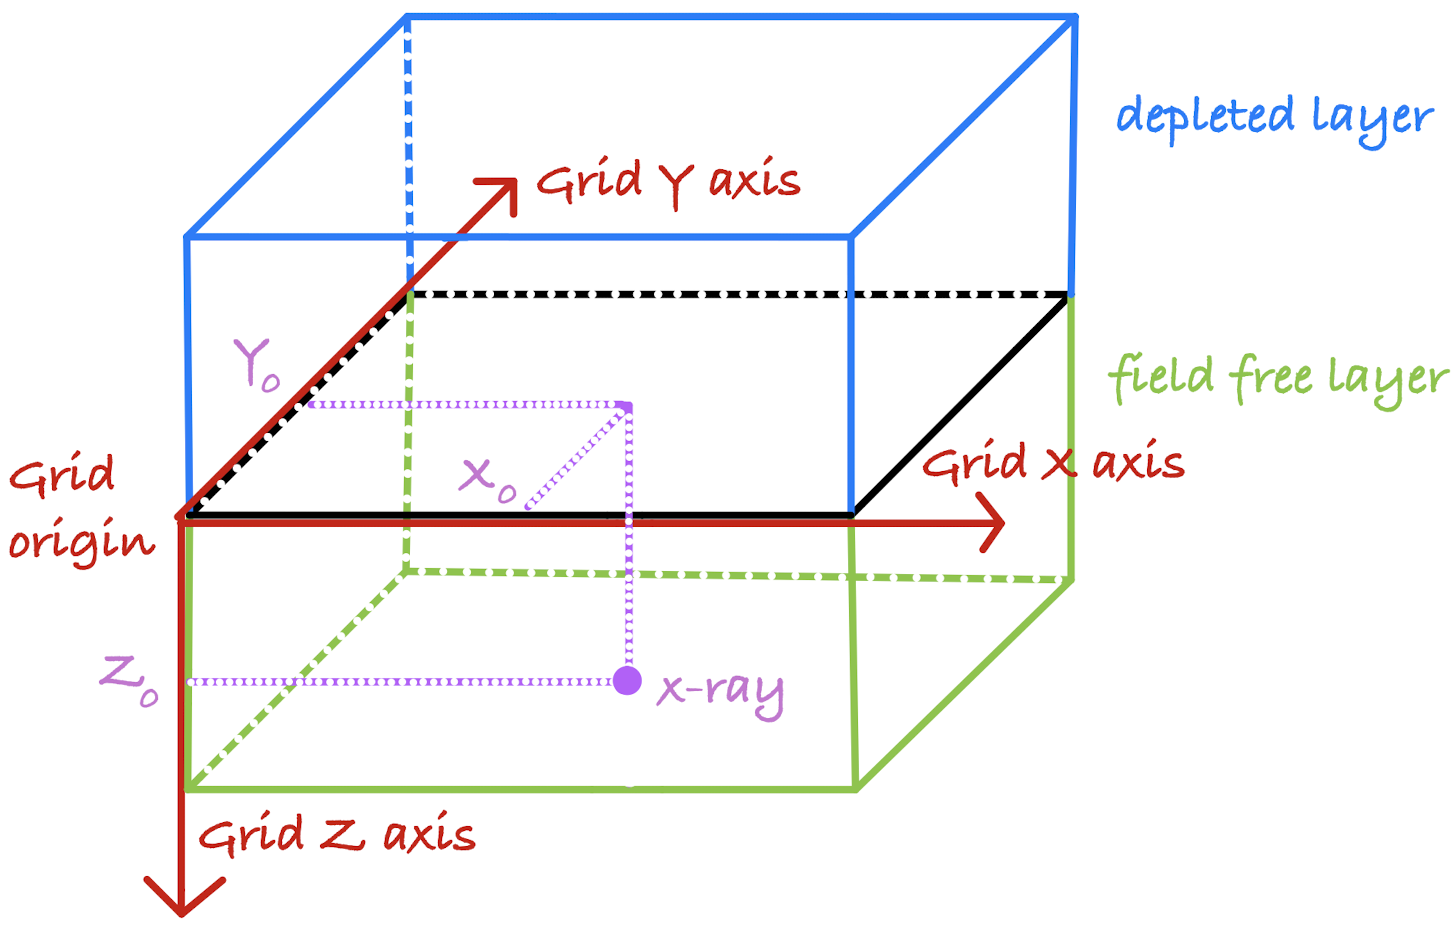
\includegraphics[width=0.7\linewidth]{images/layers.png}
    \caption{Layers of CCD with the initial interaction point $(x_0, y_0, z_0)$ of the x-ray}
    \label{fig:layers}
\end{figure}

Over time, more accurate variations of CCDs such as EMCCDs were developed. An EMCCD is more accurate than an CCD because it reduces the amount of noise by amplifying the charge before converting it to voltage and generating the image.


%%%%%%%%%%%
\subsection{Mathematics of EMCCDs}
An EMCCD camera produces a black and white pixelated image such as the one in the Figure \ref{fig:emccd}. The whiter a pixel is, the more charge was detected in the pixel by the camera. Therefore, the whiter spots in the image are the spots where the x-ray hit.

\begin{figure}[H]
    \centering
    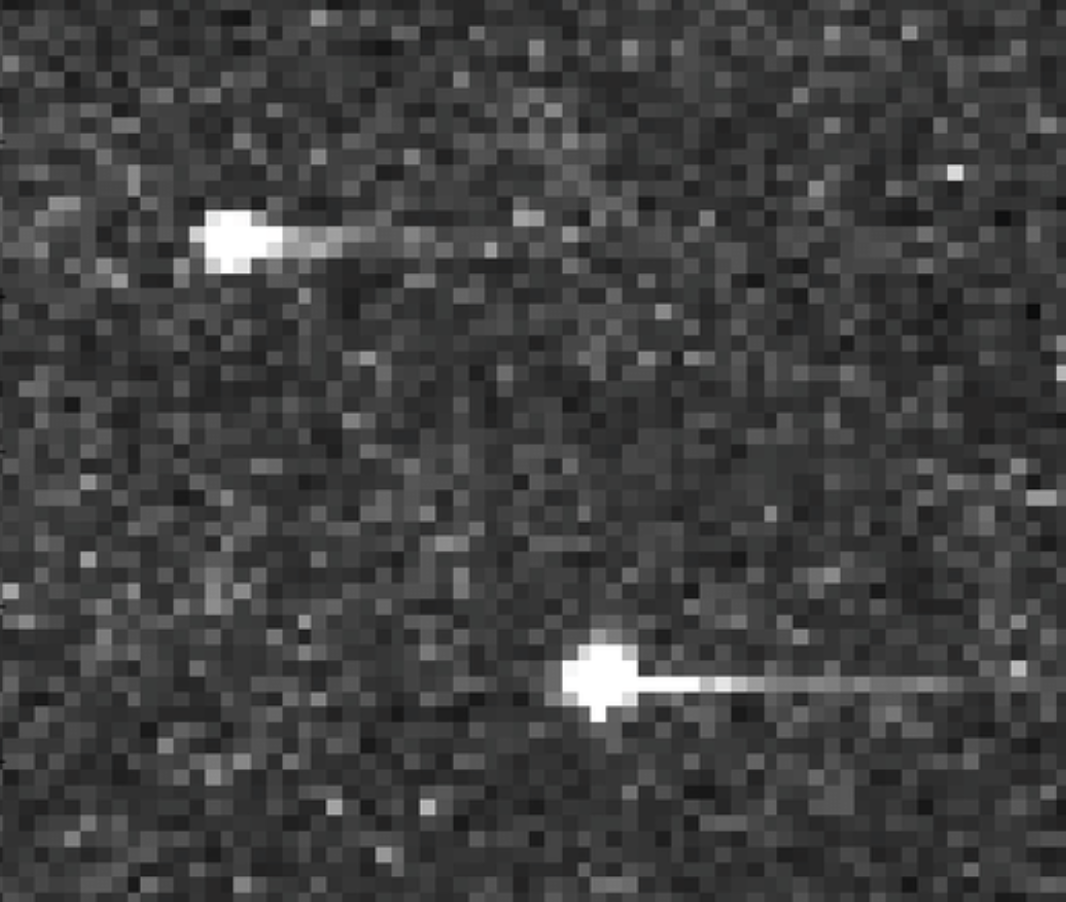
\includegraphics[width=0.6\linewidth]{images/emccd.png}
    \caption{Image produced by EMCCDs}
    \label{fig:emccd}
\end{figure}

The x-ray hits the pixelated grid of EMCCD at the initial point $(x_0, y_0, z_0)$ as shown in Figure \ref{fig:layers}. The variables $x_0$ and $y_0$ are coordinates that gives us the position on the pixelated grid. The variable $z_0$ tells us how deep the x-ray hit the pixel. If $z_0=0$, the x-ray hit the pixel on its surface and if $z=1$, the x-ray hit the pixel at the maximum depth below its surface.

We can calculate a theoretical charge accumulated in each pixel in the grid of EMCCD using the following formula [2] where $x = [b_i, b_{i+1}]$ and $y = [c_j, c_{j+1}]$ are pixel borders.

\begin{equation} 
\label{eq:q}
q_{ij} =    
 2 \sum\limits_{n=0}^\infty 
 \alpha_n  \cdot \sin(\alpha_n z_0)
  \int \limits_{0} ^\infty    \exp \left( - \frac{\alpha_n^2}{2} \sigma^2 \right) 
  \frac{1}{\pi}  \int \limits_{b_i} ^{b_{i+1}}  \int \limits_{c_j} ^{c_{j+1}}   
  \exp \left(  - \frac{r^2}{2 \sigma^2} \right) 
\frac{dx}{\sqrt{2}\sigma} \cdot \frac{dy} {\sqrt{2} \sigma} \cdot \frac{d\sigma^2}{2}
\end{equation}


%%%%%%%%%%%%%%%%%%%%%%%%%%%%%%%%%%%%%%%%%%%%%%%%%%%%%%%%%%%%%%%%%
\section{Computing Theoretical Charge Distribution}

The charge $q_{ij}$ in Equation \ref{eq:q} cannot be computed using any analytical methods, but it can be accurately estimated by numerical calculations performed by our $\text{Qint\_main.cpp}$ program.

\subsection{Executing Program}
The Figure \ref{fig:program} contains the commands for compiling and executing the program using the root environment in the command line.

\begin{figure}[H]
    \centering
    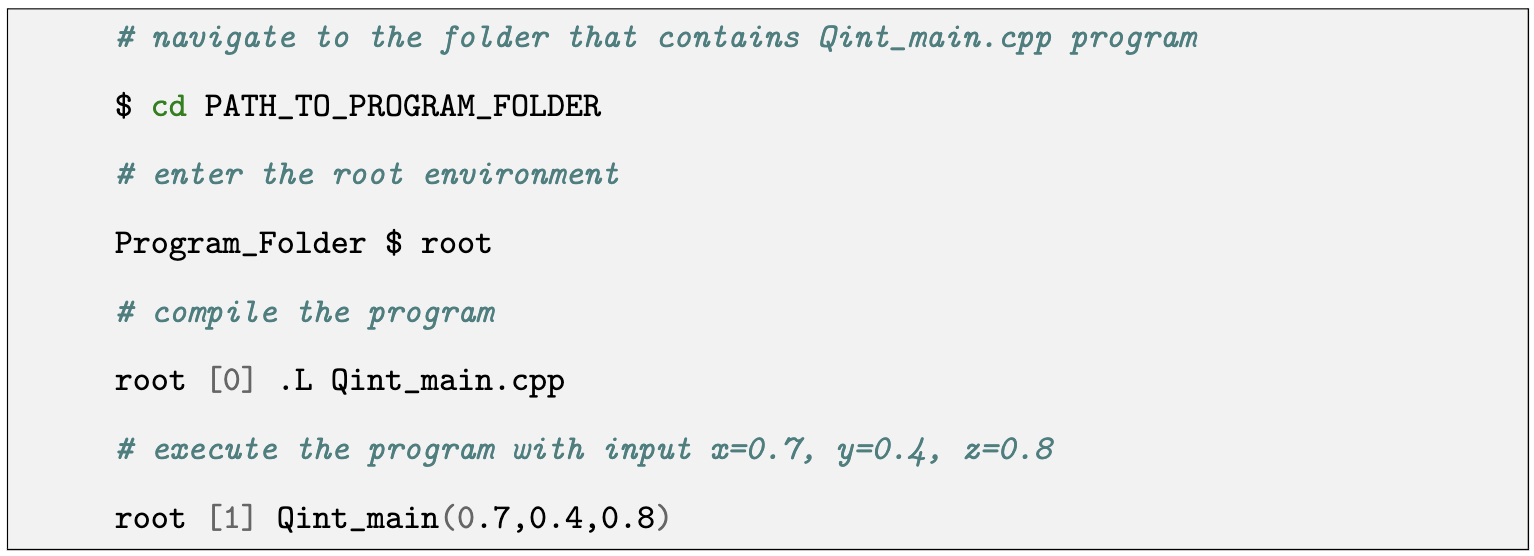
\includegraphics[width=1\linewidth]{images/program.png}
    \caption{Executing the Qint\_main.cpp program on MacOS}
    \label{fig:program}
\end{figure}

%\begin{mdframed}[backgroundcolor=bg]
%\begin{minted}[]{bash}
%    # navigate to the folder that contains Qint_main.cpp program
%    $ cd PATH_TO_PROGRAM_FOLDER
%    # enter the root environment
%    Program_Folder $ root
%    # compile the program
%    root [0] .L Qint_main.cpp
%    # execute the program with input x=0.7, y=0.4, z=0.8
%    root [1] Qint_main(0.7,0.4,0.8)
%\end{minted}
%\end{mdframed}

\subsection{Inputs and Outputs of Program}

In order to understand the inputs and outputs of the program, we have to explain the two coordinate systems of a pixelated grid of CCD. There is one coordinate system for the whole pixelated grid as shown in Figure \ref{fig:grid} and another coordinate system for each individual pixel as shown in Figure \ref{fig:pixel}. 

\begin{figure}[H]
\centering
\begin{subfigure}{.5\textwidth}
  \centering
  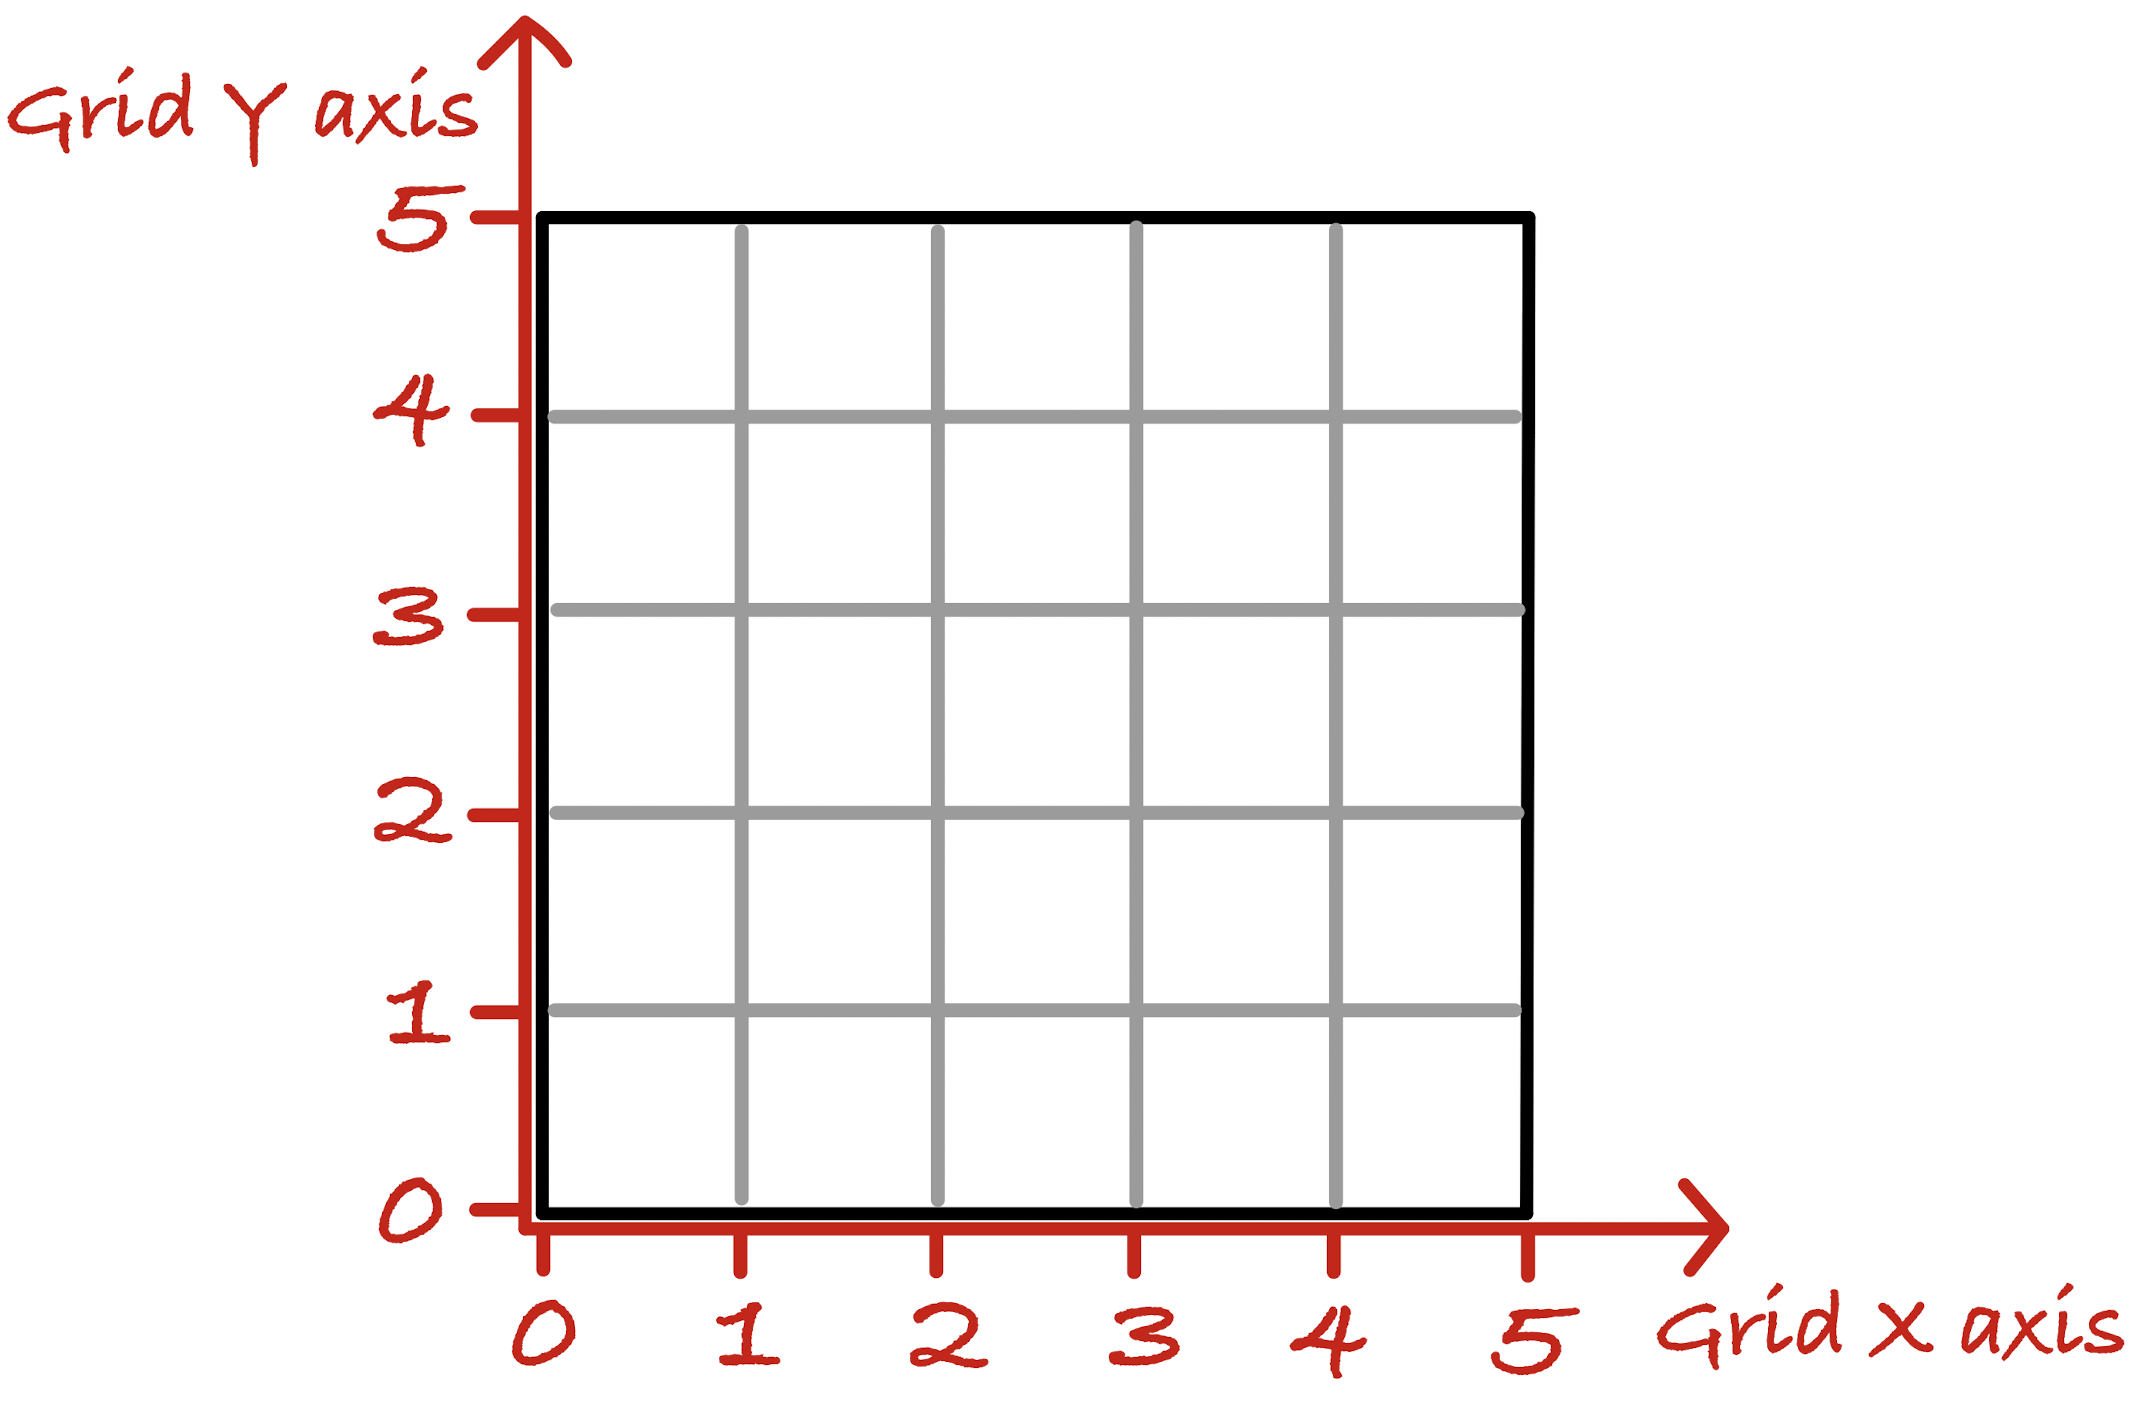
\includegraphics[width=1\linewidth]{images/grid1.png}
  \caption{The grid coordinate system of the CCD}
  \label{fig:grid}
\end{subfigure}%
\begin{subfigure}{.5\textwidth}
  \centering
  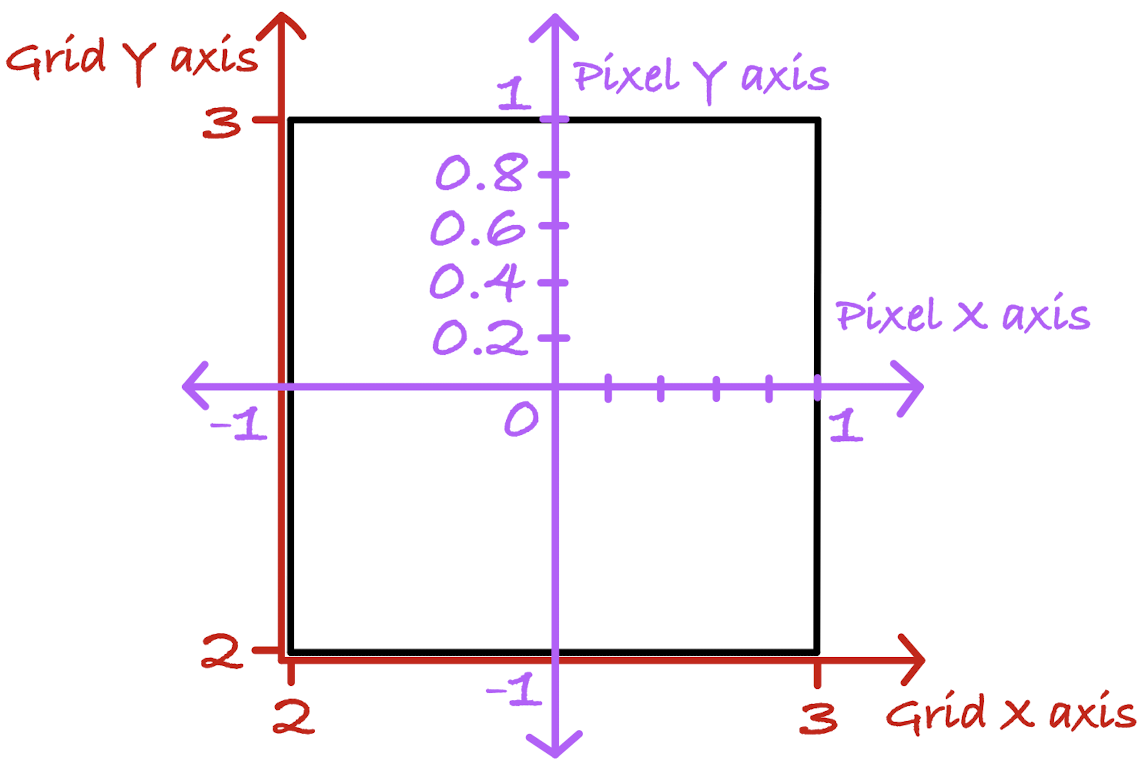
\includegraphics[width=1\linewidth]{images/grid2.png}
  \caption{The pixel coordinate system of each pixel}
  \label{fig:pixel}
\end{subfigure}
\caption{The coordinate system of a pixelated grid of CCD}
\label{fig:test}
\end{figure}

The program takes three parameters $x,y,z$ that specify the original x-ray coordinate in a central pixel in the $5\times 5$ grid using the pixel coordinate system. As we can see from the \ref{fig:pixel}, the constraints for the inputs are $-1\leq x \leq 1$, $-1\leq y \leq 1$, and $-1\leq z \leq 1$. It outputs a graph of the charge distribution over the $5\times 5$ grid such as the ones in Figure \ref{fig:q}.


\section{Symmetry of the Pixelated Grid}
The program generates the charge distribution for an original x-ray position that is located at the center pixel of the $5\times 5$ grid. Note that the grid is symmetric by its center. This means that when we rotate the charge distribution corresponding to the original x-ray coordinate $(x,y)$ by 90°, 180°, and 270° counterclockwise, we will get the same distribution corresponding to original x-ray coordinate $(-y,x)$, $(-x,y)$, and $(y,-x)$ as shown in Figure \ref{fig:q}.


%Therefore, charge distributions for all possible original x-ray coordinates can be obtained just by generating the distributions for all x-ray positions in the first quadrant of the central pixel ($0\leq x \leq 1$ and $0\leq y \leq 1$ in the pixel coordinate system). That is because 

\begin{figure}[H]
    \centering
    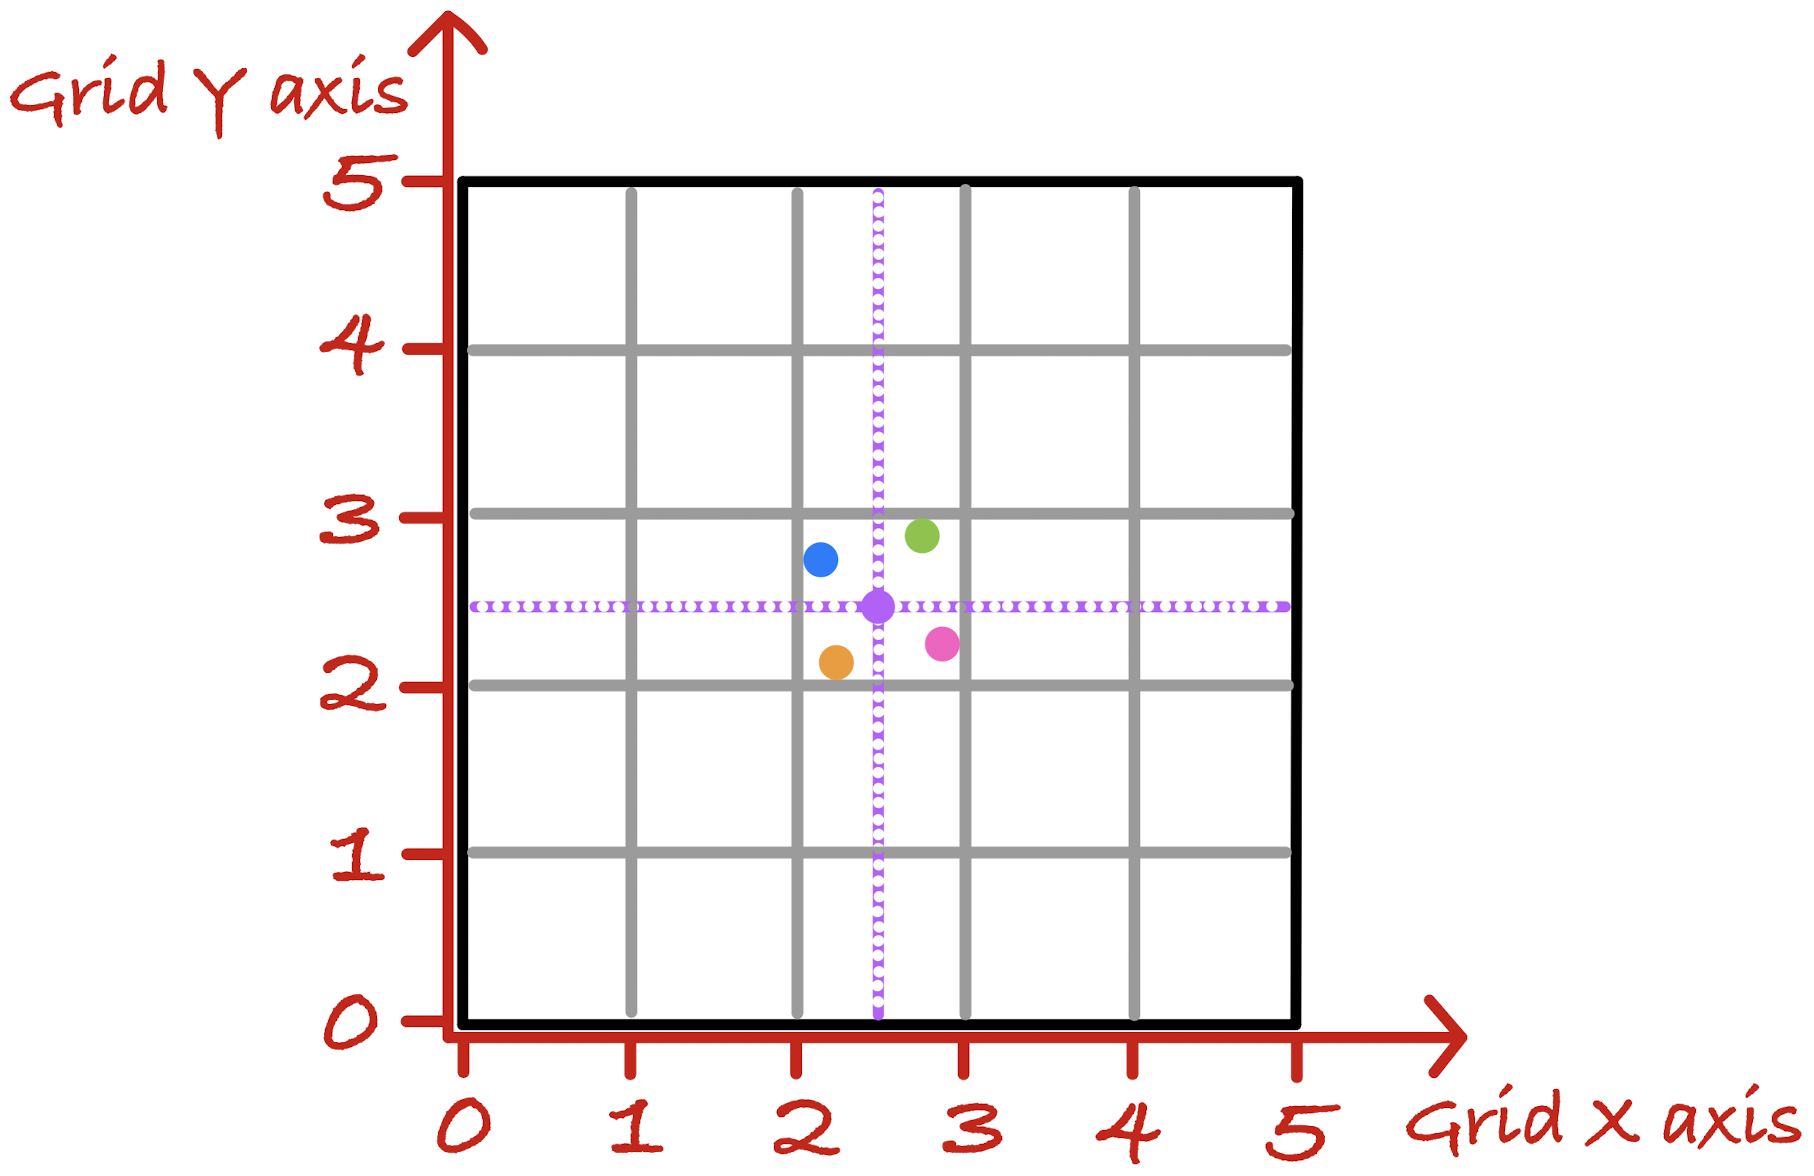
\includegraphics[width=0.8\linewidth]{images/rotation.png}
    \caption{All points shown will have the same charge distribution that differs only by rotation}
    \label{fig:symmetry}
\end{figure}



\begin{figure}[H]
\centering
\begin{subfigure}{.5\textwidth}
  \centering
  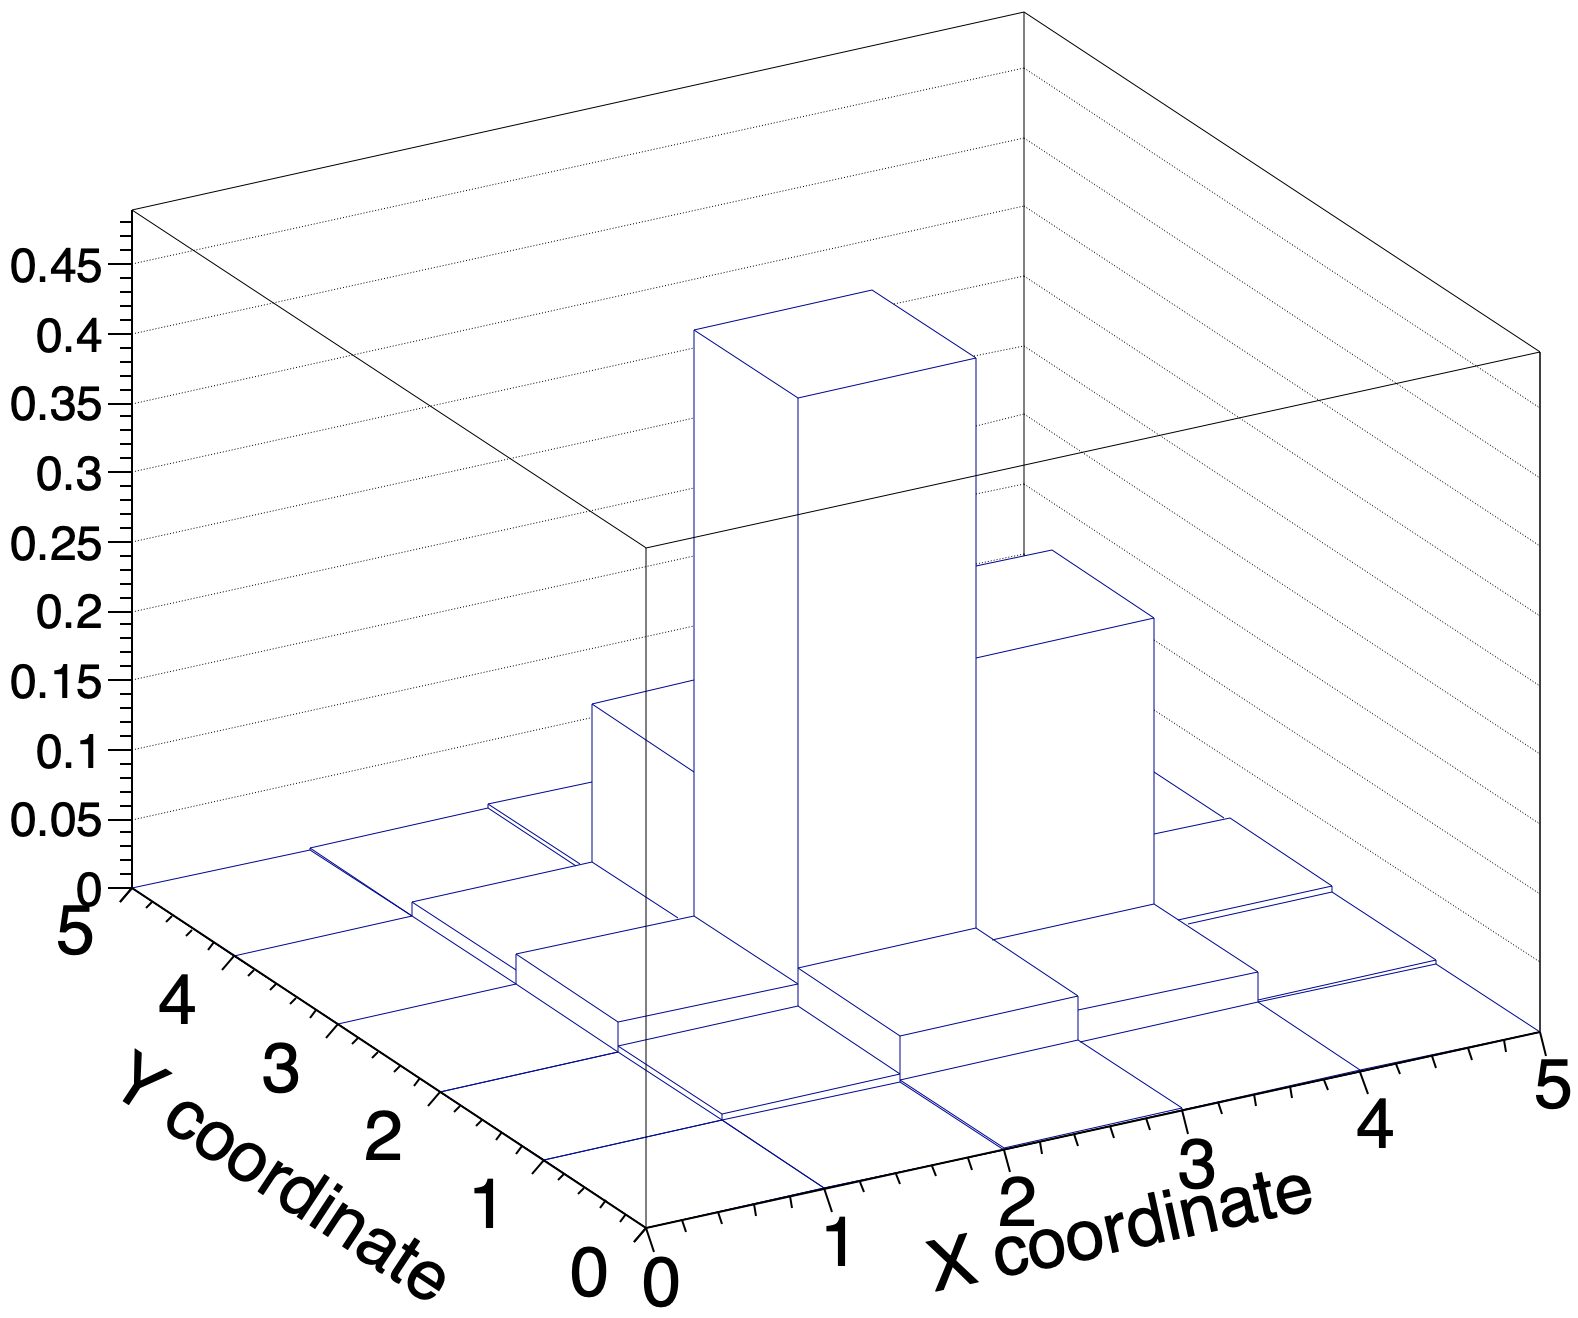
\includegraphics[width=.9\linewidth]{images/q1.png}
  \caption{$x=0.7$ and $y=0.4$\\no rotation}
  \label{fig:q1}
\end{subfigure}%
\begin{subfigure}{.5\textwidth}
  \centering
  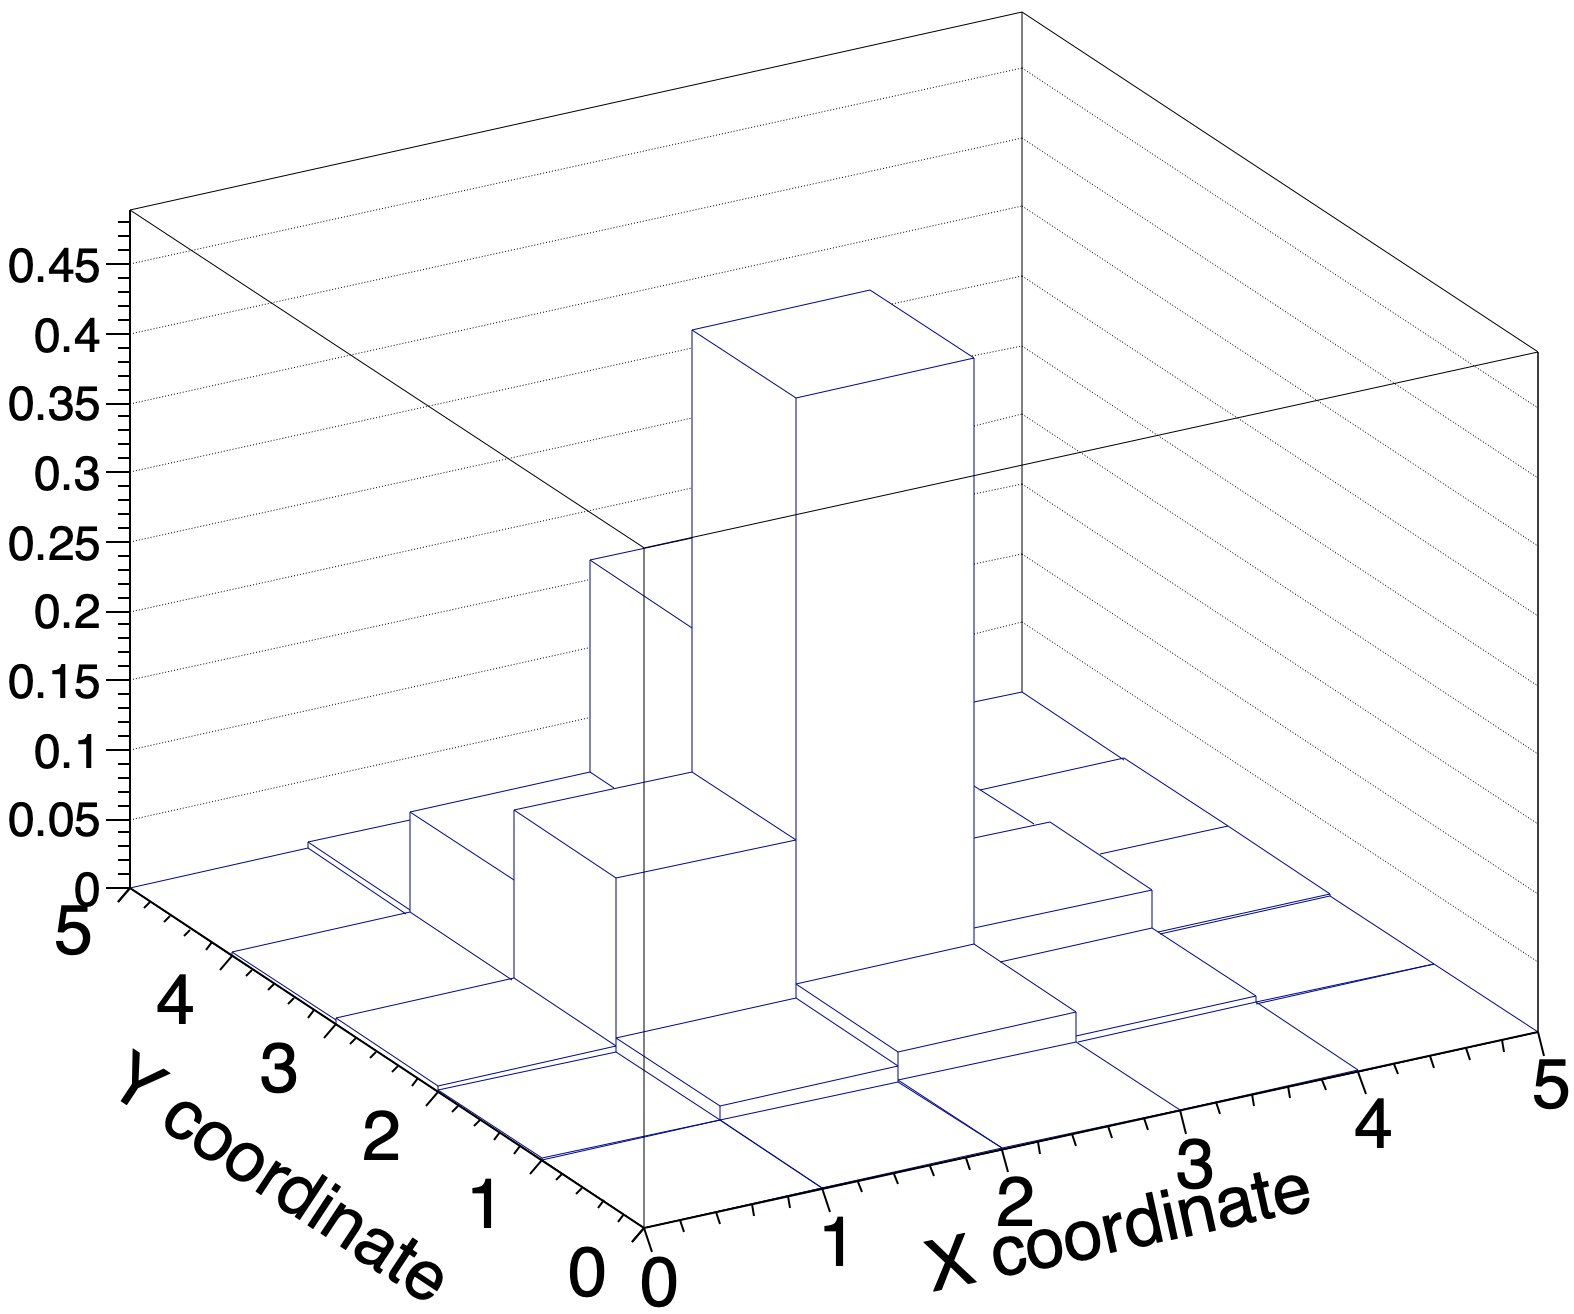
\includegraphics[width=.9\linewidth]{images/q2.png}
  \caption{$x=-0.4$ and $y=0.7$\\90° counterclockwise rotation}
  \label{fig:q2}
\end{subfigure}
\begin{subfigure}{.5\textwidth}
  \centering
  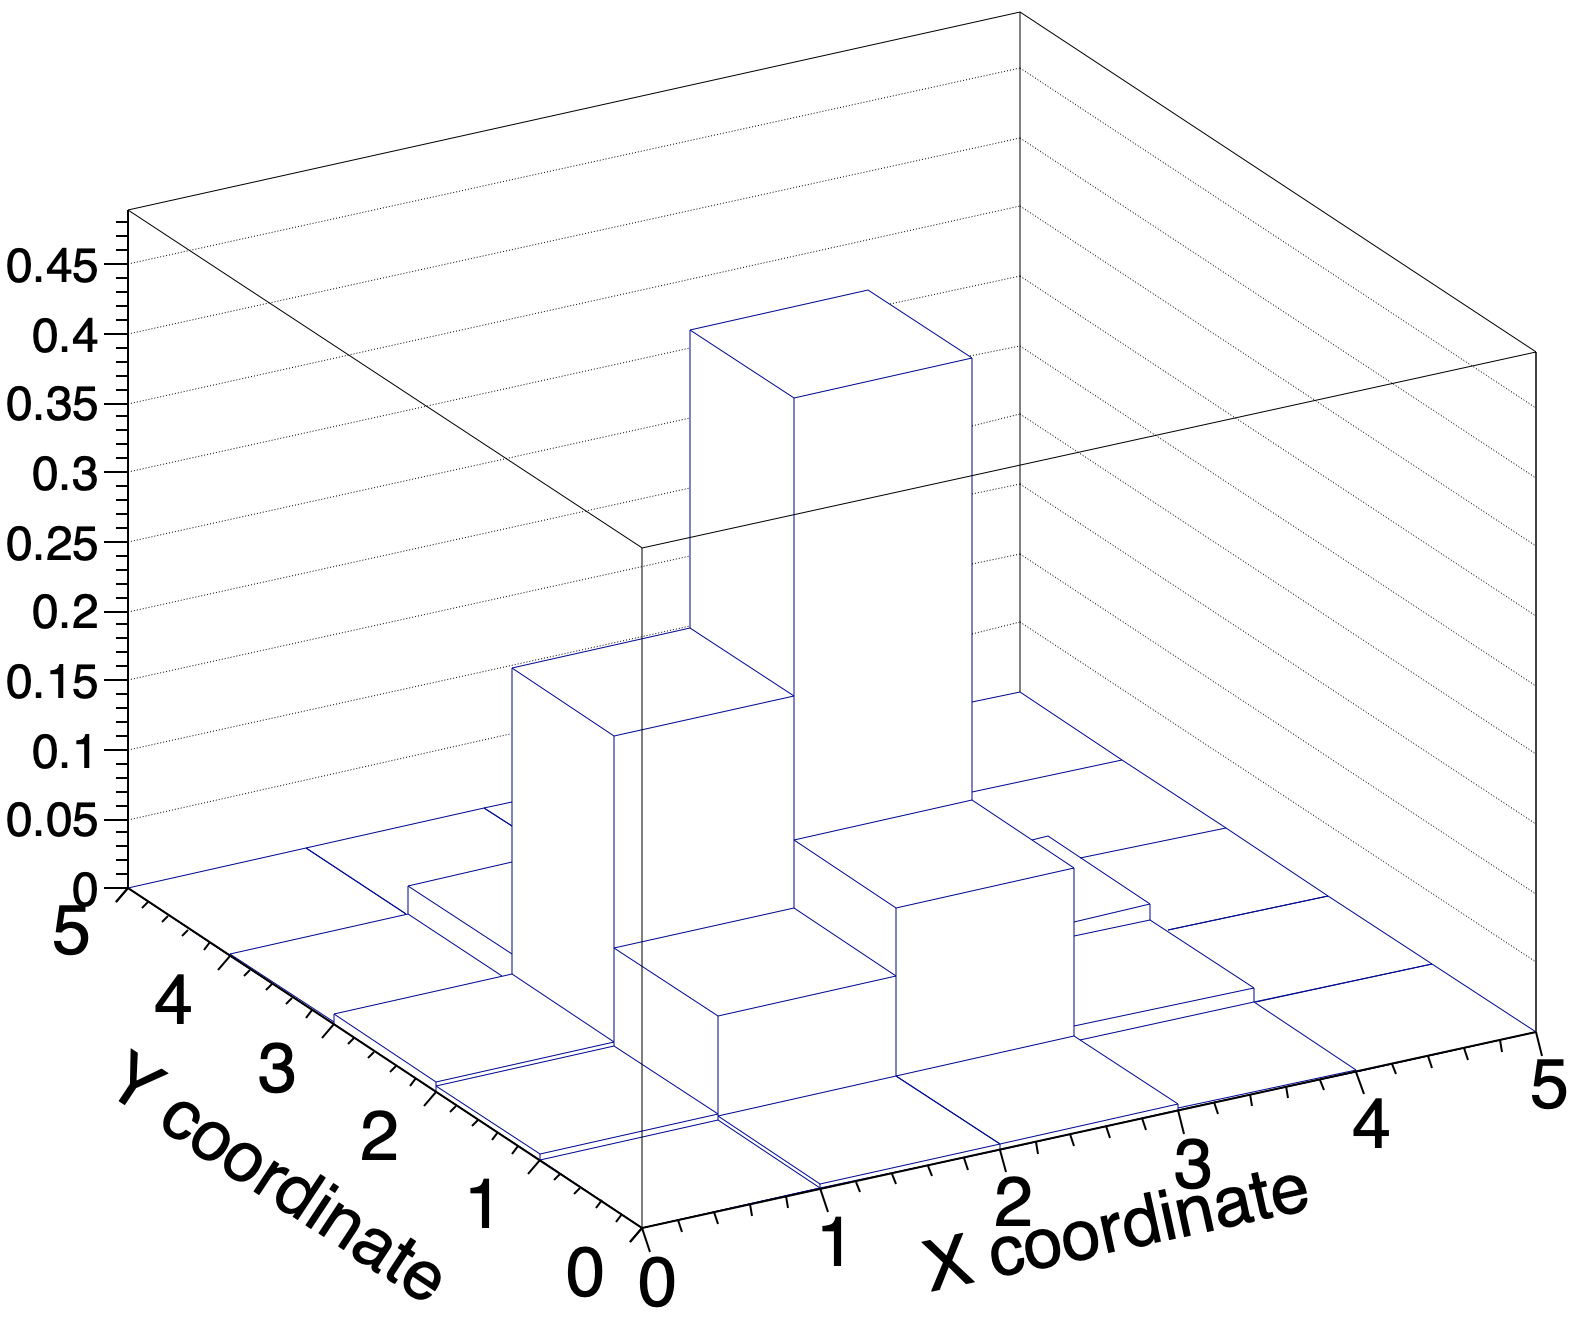
\includegraphics[width=.9\linewidth]{images/q3.png}
  \caption{$x=-0.7$ and $y=-0.4$\\180° counterclockwise rotation}
  \label{fig:q3}
\end{subfigure}%
\begin{subfigure}{.5\textwidth}
  \centering
  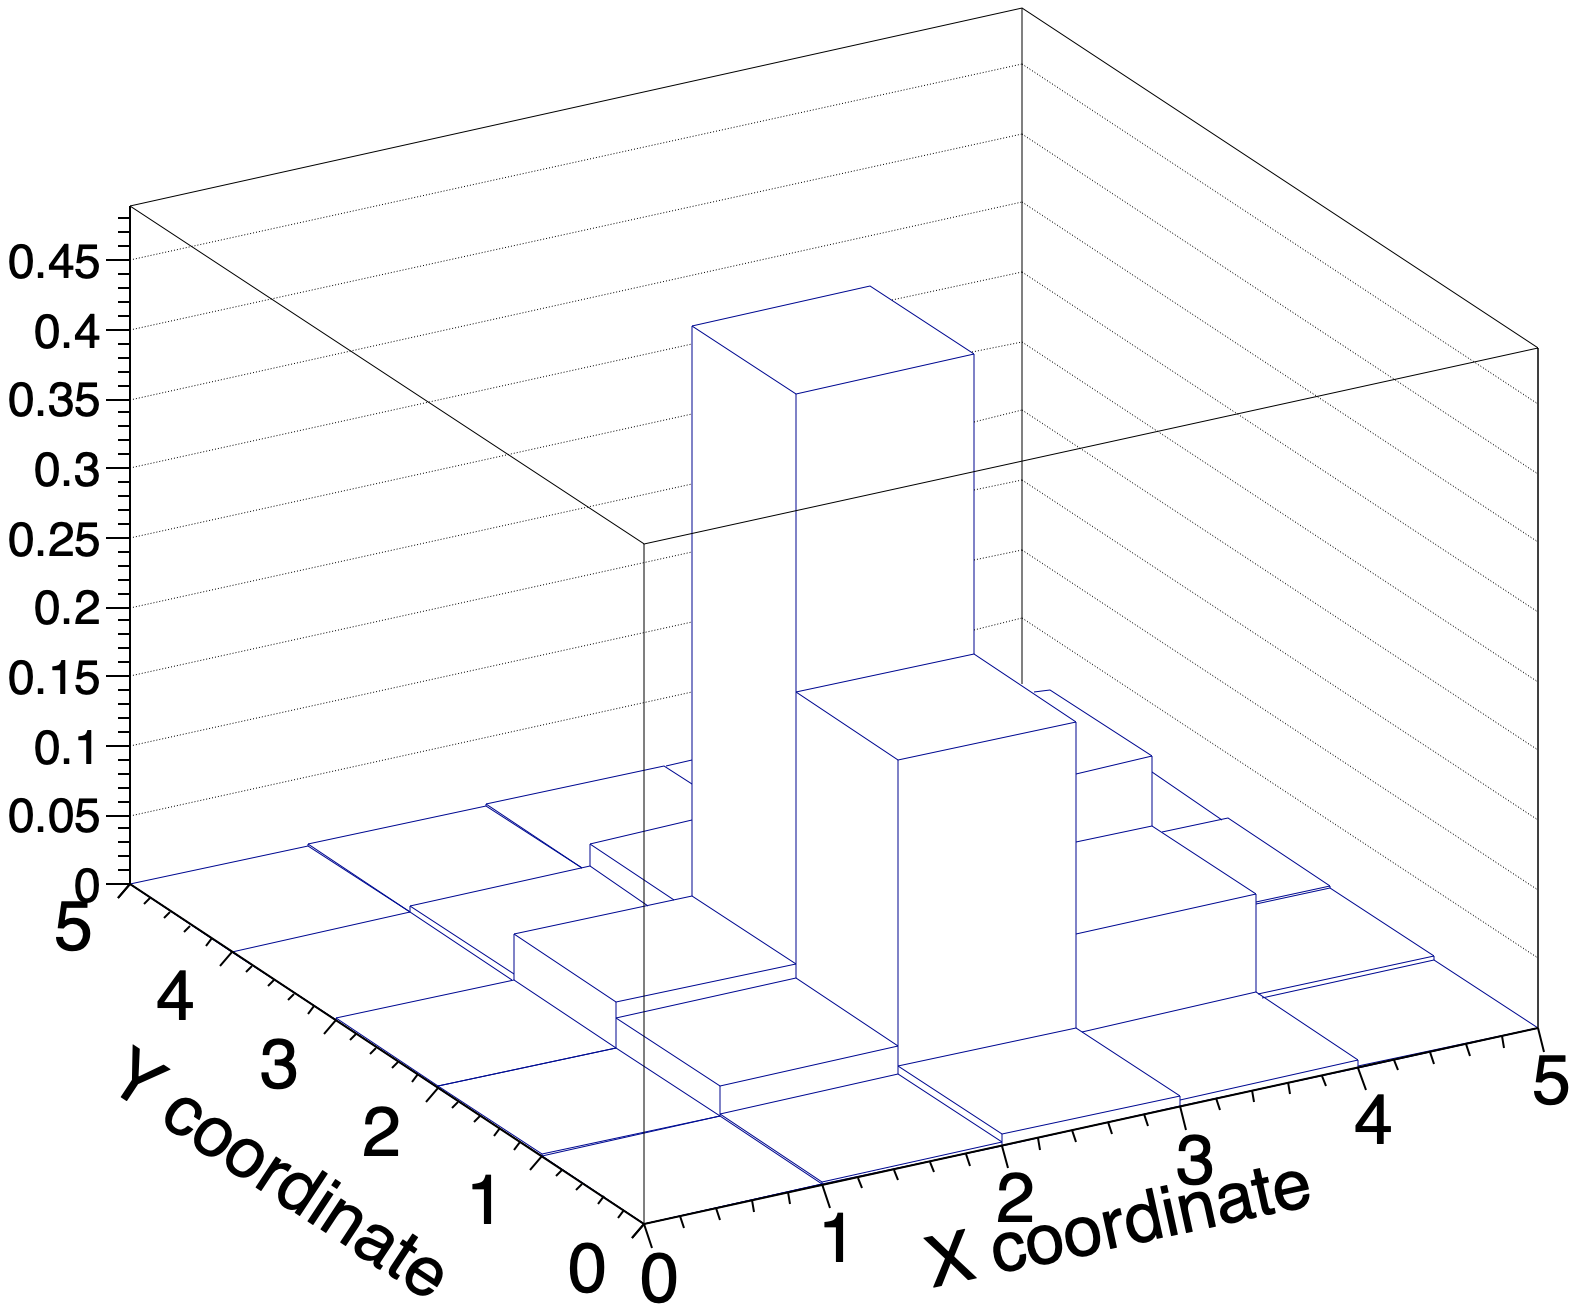
\includegraphics[width=.9\linewidth]{images/q4.png}
  \caption{$x=0.4$ and $y=-0.7$\\270° counterclockwise rotation}
  \label{fig:q4}
\end{subfigure}
\caption{Symmetry of the charge distribution for the original x-ray pixel coordinate $x=0.7$ and $y=0.4$}
\label{fig:q}
\end{figure}

%%%%%%%%%%%%%%%%%%%%%%%%%%%%%%%%%%%%%%%%%%%%%%%%%%%%%%%%%%%%%%%%%
%%%%%%%%%%%%%%%%%%%%%%%%%%%%%%%%%%%%%%%%%%%%%%%%%%%%%%%%%%%%%%%%%
\section{The Model of Charge Distribution}
Our goal is to find an accurate model that can accurately predict the original $x$ and $y$ coordinate of the x-ray given the charge distribution over the pixelated grid of CCD.

%%%%%%%%%%%
\subsection{The Model}
In the Figure \ref{fig:charge}, we can see the charge distribution that we have computed using the formula \ref{eq:q} for the original x-ray coordinate $x=2.9$ and $y=2.7$. How can we obtain the original coordinate just based on the distribution?

%Qint_main(0.7,0.4,0.8)
\begin{figure}[H]
    \centering
    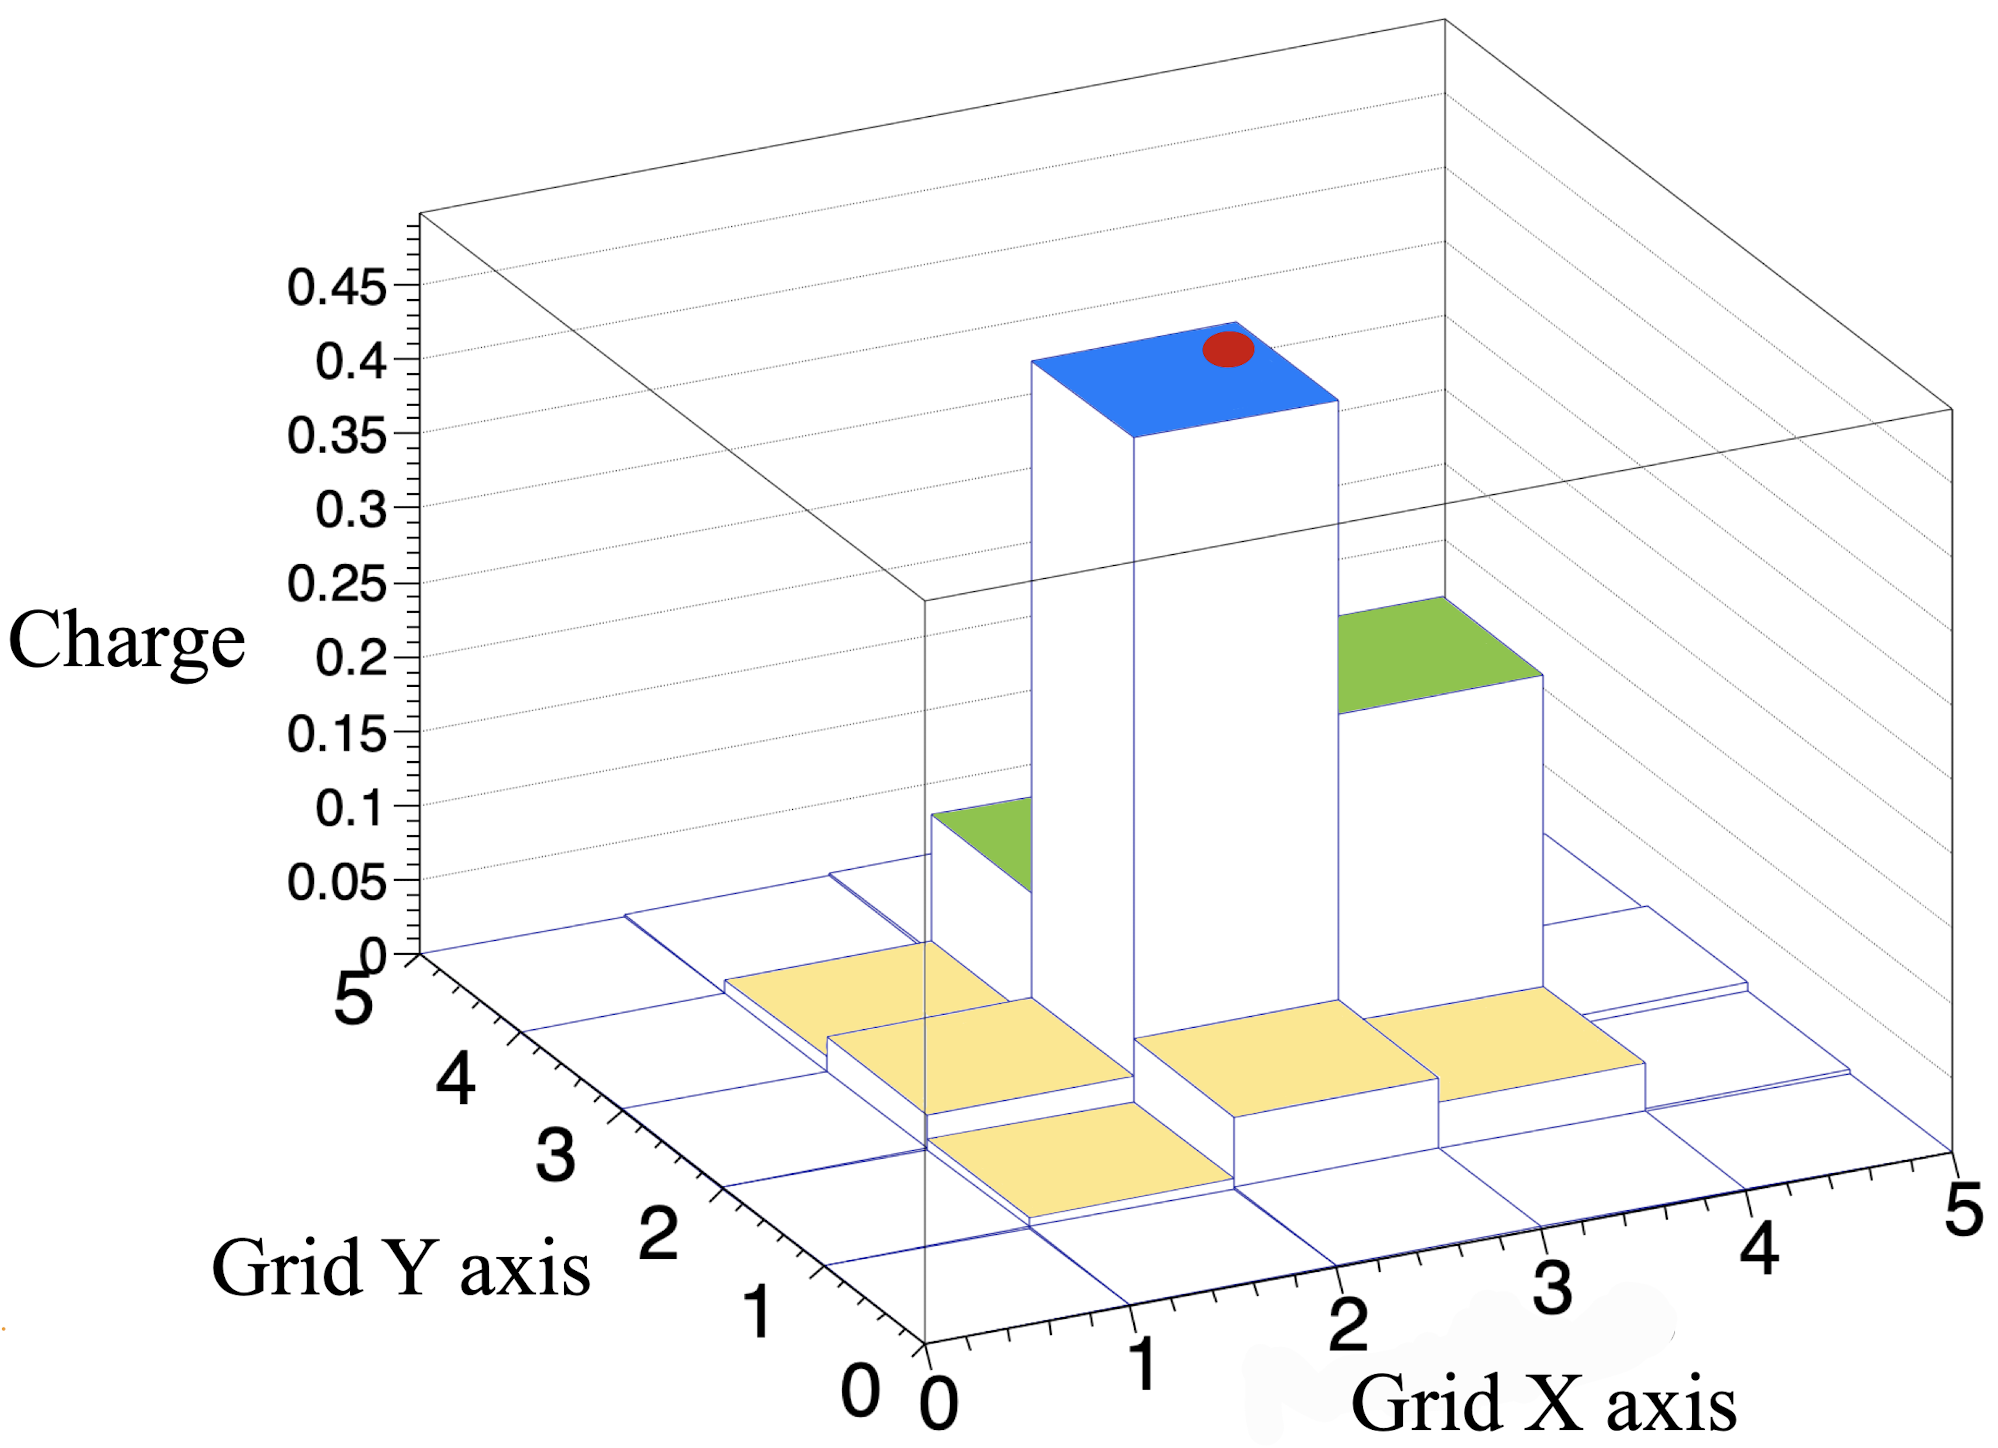
\includegraphics[width=0.7\linewidth]{images/charge_distribution.png}
    \caption{Charge distribution for the original x-ray coordinate $x=2.9$ and $y=2.7$.}
    \label{fig:charge}
\end{figure}

We can intuitively see which pixel the x-ray hit. The x-ray hit the pixel in the middle of the grid at the position $x=2$ and $y=2$ because this pixel accumulated the most charge. We can also tell that the x-ray hit the middle pixel at the upper right corner by looking at the neighboring pixels. We can see that the green neighboring pixels on the right accumulated more charge than the yellow pixels on the left. Therefore, the x-ray hit the pixel at a position that is closer to the green pixels than the yellow pixels. Based on this reasoning, we can guess that the original coordinate is approximately where the red dot is.

In order to formally determine the original x-ray coordinate, we need to fit a model to our charge distribution using the least squares method. We have chosen two-dimensional Gaussian model which is defined by five parameters - the height of its peak, $x$ and $y$ coordinates of its peak, and the width of the bell in the $x$ and $y$ direction. The position of the peak is an estimate of the original x-ray coordinate because the peak accumulated the most charge.

In Figure \ref{fig:model}, we can see the mathematically computed and fitted charge distribution. The position of the fitted peak is $x=2.872$ and $y=2.673$ which is very close to the original x-ray coordinate which is $x=2.9$ and $y=2.7$. Furthermore, in Figure \ref{fig:model}, we can see that our model has very low prediction errors (less than 20\%) around the middle pixel where the x-ray hit. Therefore, we can see that our model is accurate in this case.

\begin{figure}[H]
\centering
\begin{subfigure}{.5\textwidth}
  \centering
  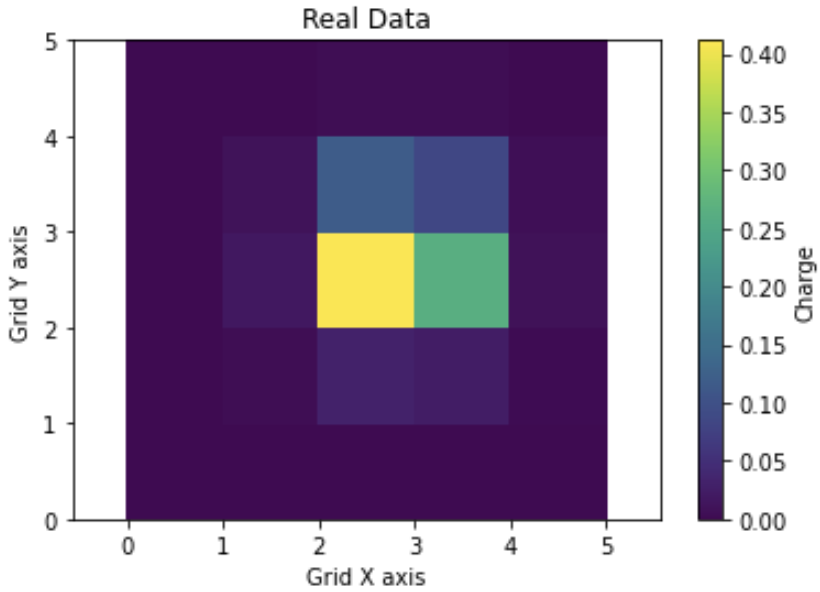
\includegraphics[width=.9\linewidth]{images/real.png}
  \caption{Charge distribution computed by the formula}
  \label{fig:sub1}
\end{subfigure}%
\begin{subfigure}{.5\textwidth}
  \centering
  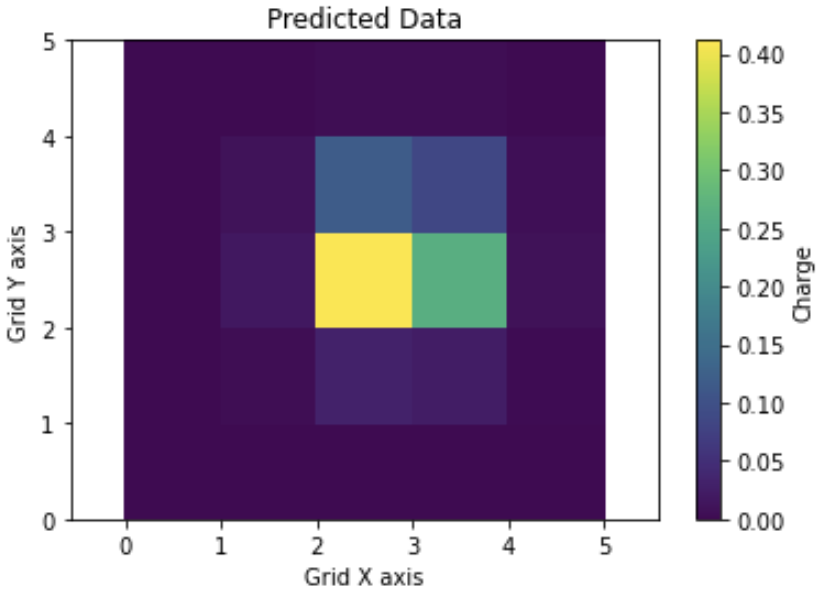
\includegraphics[width=.9\linewidth]{images/predicted.png}
  \caption{Charge distribution predicted by the model}
  \label{fig:sub2}
\end{subfigure}
\caption{Charge distributions}
\label{fig:model}
\end{figure}


\begin{figure}[H]
\begin{subfigure}{.5\textwidth}
  \centering
  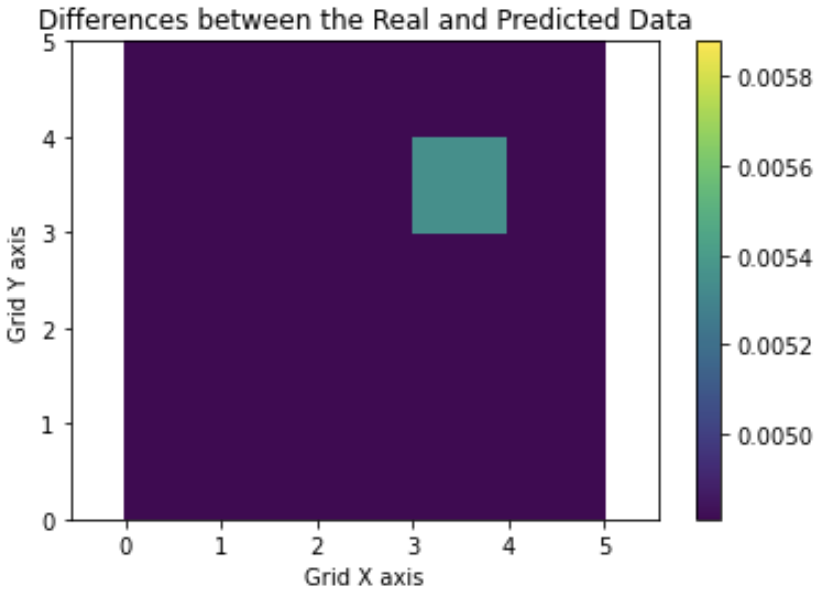
\includegraphics[width=0.9\linewidth]{images/differences.png}
  \caption{Differences between computed and predicted\\ distributions}
  \label{fig:sub1}
\end{subfigure}%
\begin{subfigure}{.5\textwidth}
  \centering
  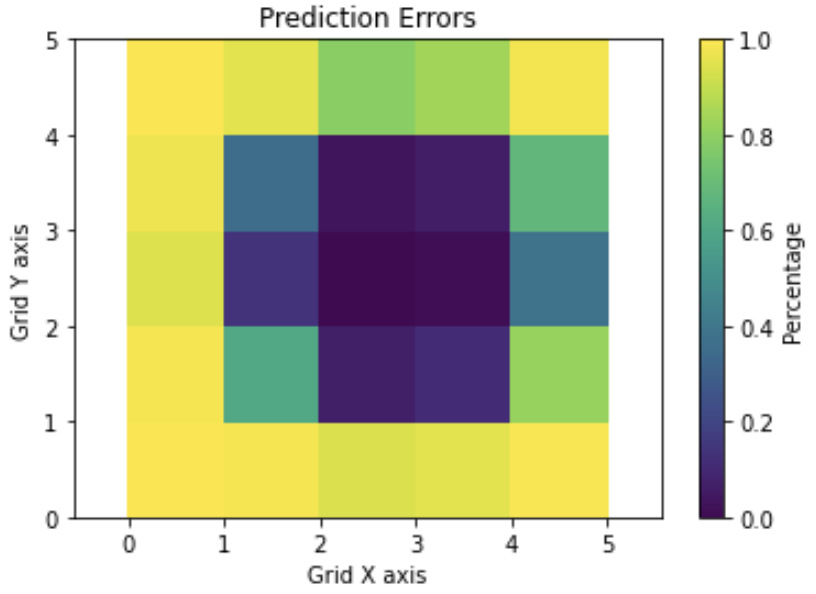
\includegraphics[width=0.9\linewidth]{images/errors.png}
  \caption{Prediction errors of the model (errors larger than 1 are displayed as 1)}
  \label{fig:sub2}
\end{subfigure}
\caption{Estimating accuracy of the model}
\label{fig:accuracy}
\end{figure}

%%%%%%%%%%%
\subsection{The Accuracy of the Model}
We want to estimate the accuracy of our two-dimensional Gaussian distribution model for every possible original x-ray position. Because of the symmetry of the grid explained in the previous section, we only have to fit our model to the original x-ray positions that are in the first quadrant of the middle pixel of the $5\times 5$ grid. Models for other original x-ray positions can be obtained by rotating or shifting the grid.

Since there are infinitely many original x-ray positions in the first quadrant, we have decided to take a sample of positions using $\Delta x = 0.1$, $\Delta y = 0.1$, and $\Delta z = 0.1$ as shown in the Figure \ref{fig:positions}. That gives us $11\cdot 11\cdot 11 = 1331$ original x-ray positions.

\begin{figure}[H]
    \centering
    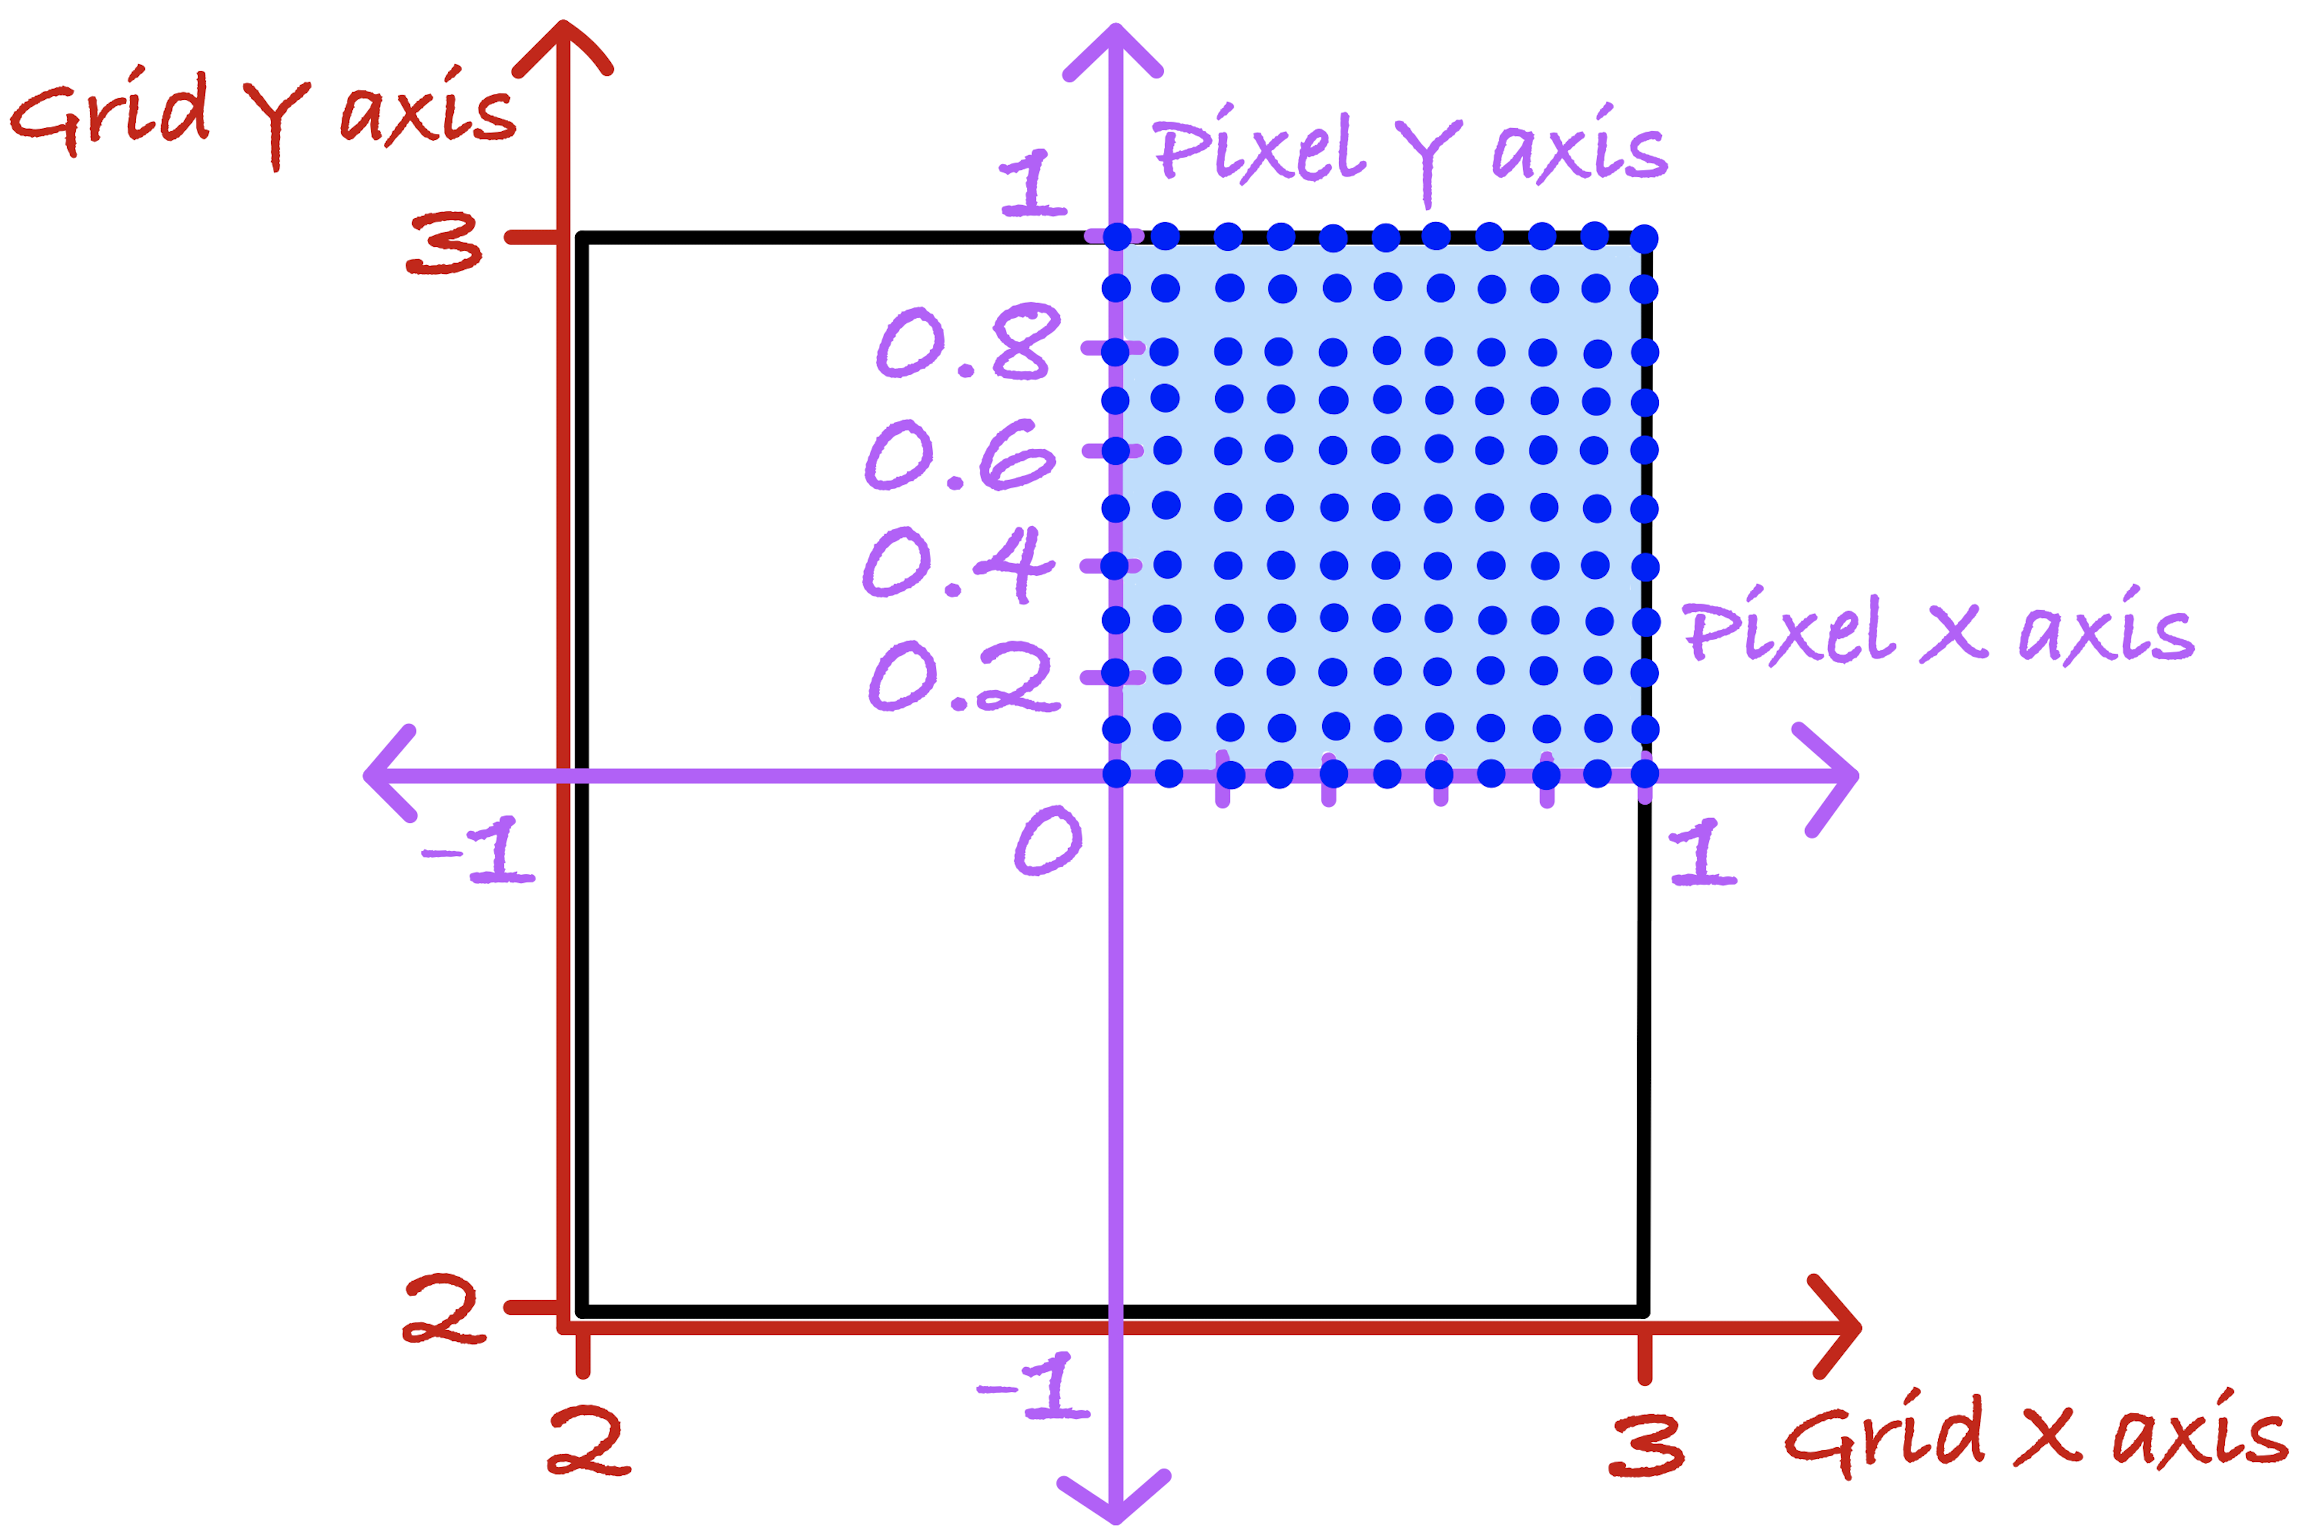
\includegraphics[width=0.7\linewidth]{images/positions.png}
    \caption{Blue dots show all original x-ray positions for the model}
    \label{fig:positions}
\end{figure}

A good way to estimate accuracy of our model is to measure the distance between the original x-ray position $(x_o,y_o)$ and the predicted x-ray position $(x_p, y_p)$. We can compute the distance using the following formula: $\sqrt{(x_o-x_p)^2 + (y_o-y_p)^2}$. We compute this distance for all 1331 original x-ray positions.

As we can see from the Figure \ref{fig:accuracy1}, our model is very accurate because the majority of distances are less than 0.1 which means that the prediction error was less than one tenth of a pixel width. 



\begin{figure}[H]
\centering
\begin{subfigure}{.5\textwidth}
  \centering
  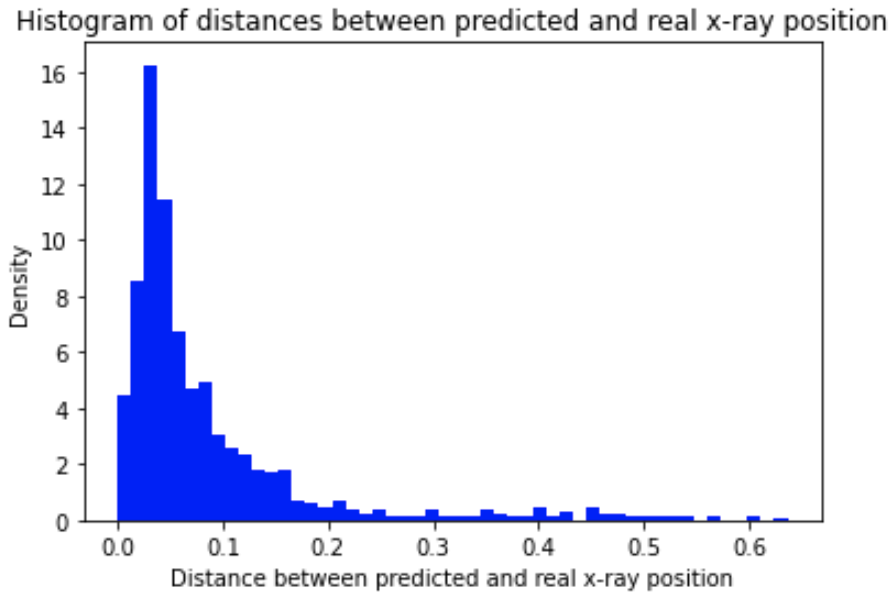
\includegraphics[width=.9\linewidth]{images/theoretical1.png}
  \caption{Charge distribution computed by the formula}
  \label{fig:accuracy1}
\end{subfigure}%
\begin{subfigure}{.5\textwidth}
  \centering
  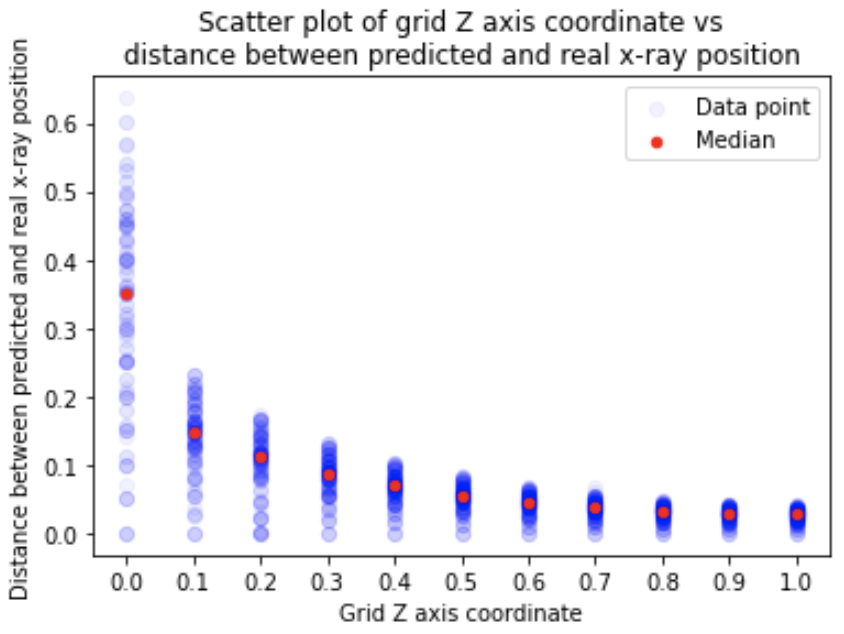
\includegraphics[width=.8\linewidth]{images/theoretical2.png}
  \caption{Charge distribution predicted by the model}
  \label{fig:accuracy2}
\end{subfigure}
\caption{Charge distributions}
\label{fig:accuracy}
\end{figure}

From the Figure \ref{fig:accuracy2}, we can also see that the accuracy of our model significantly differs based on $z$. This makes sense because the $z$ coordinate represents how deep the x-ray hit the pixel. For example, when $z=0$, the x-ray hit the pixel on the surface. This means that all charge accumulated in just one pixel and no charge accumulated in the neighboring pixels as we can see in the Figure \ref{ref:z0}, making it impossible to know where exactly the x-ray hit the pixel. On the contrary, when $z=1$, the x-ray hit the pixel at the maximum depth below its surface. Therefore, the neighboring pixels accumulated a lot of charge as we can see in the figure \ref{fig:z1}, making it easy to predict where exactly the x-ray hit the pixel by fitting the model to the distribution.


\begin{figure}[H]
\centering
\begin{subfigure}{.33\textwidth}
  \centering
  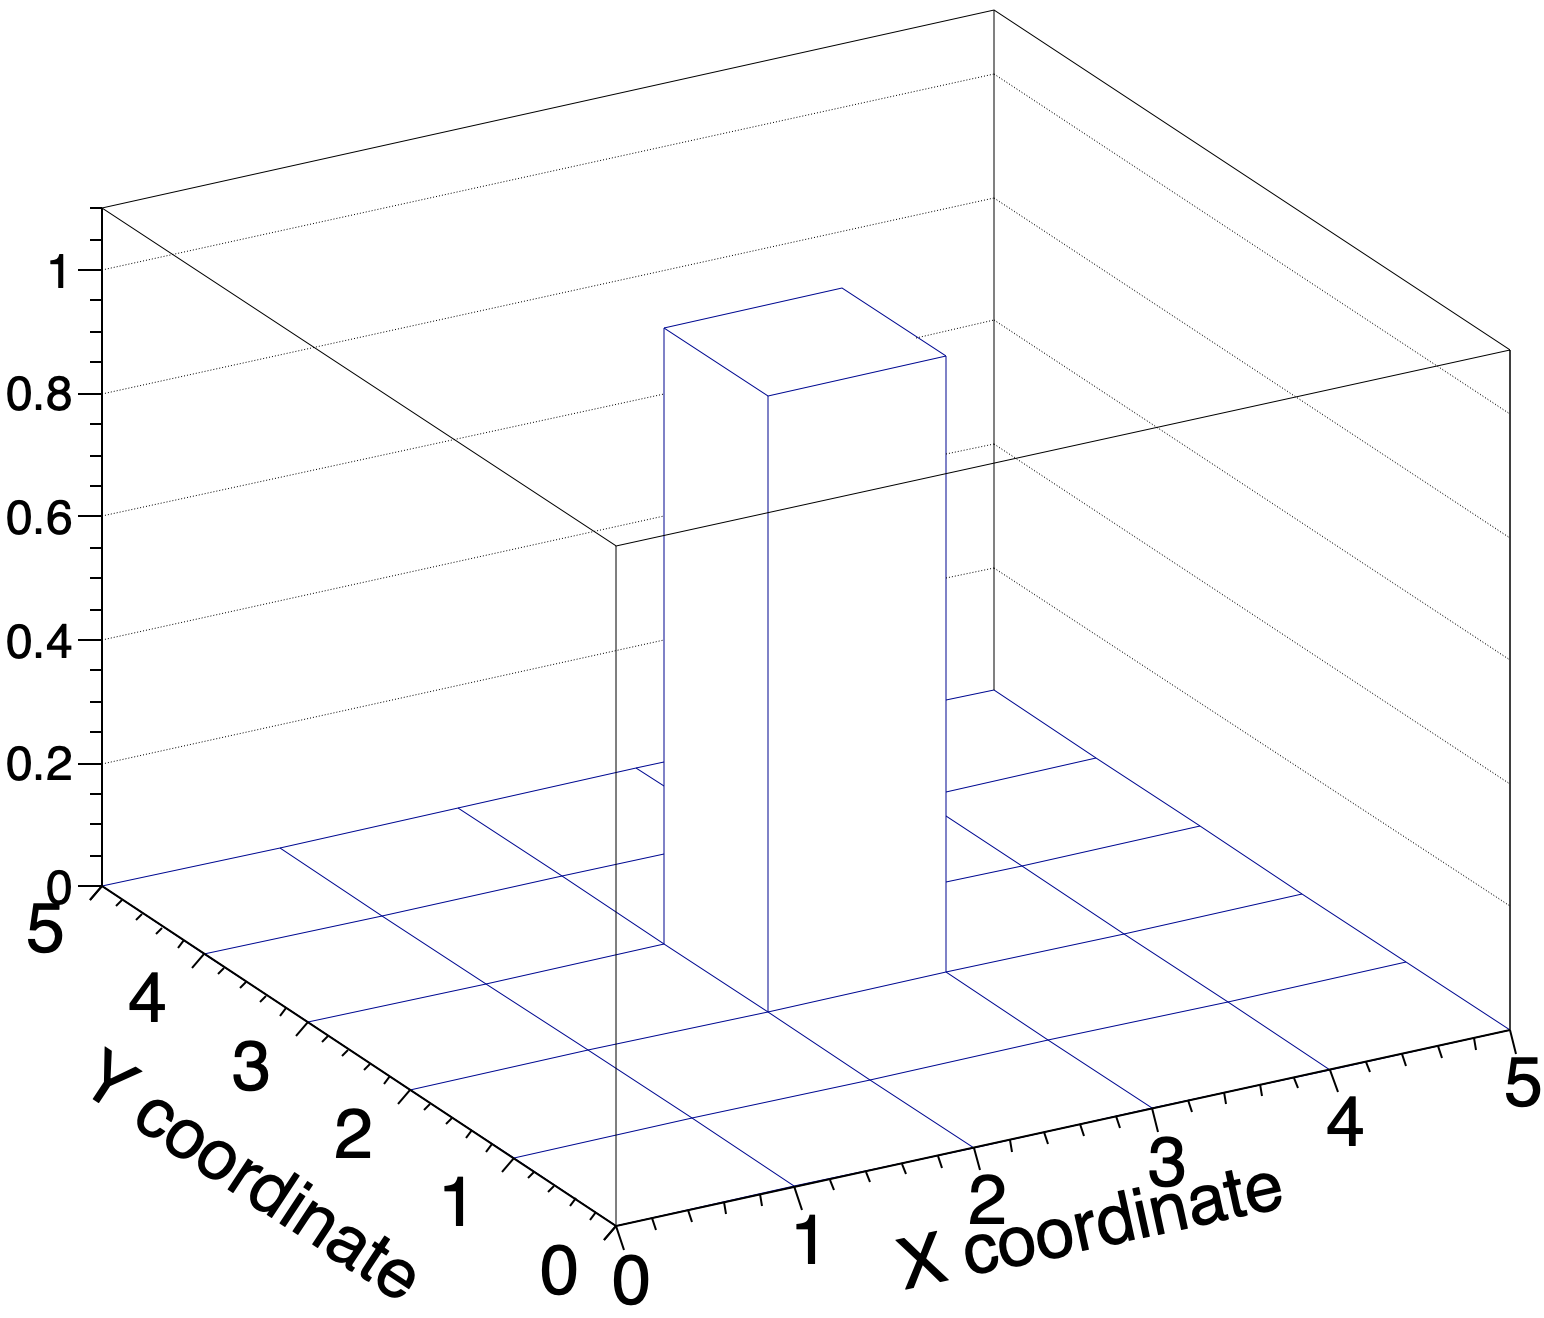
\includegraphics[width=1\linewidth]{images/z0.png}
  \caption{$z=0$}
  \label{fig:z0}
\end{subfigure}%
\begin{subfigure}{.33\textwidth}
  \centering
  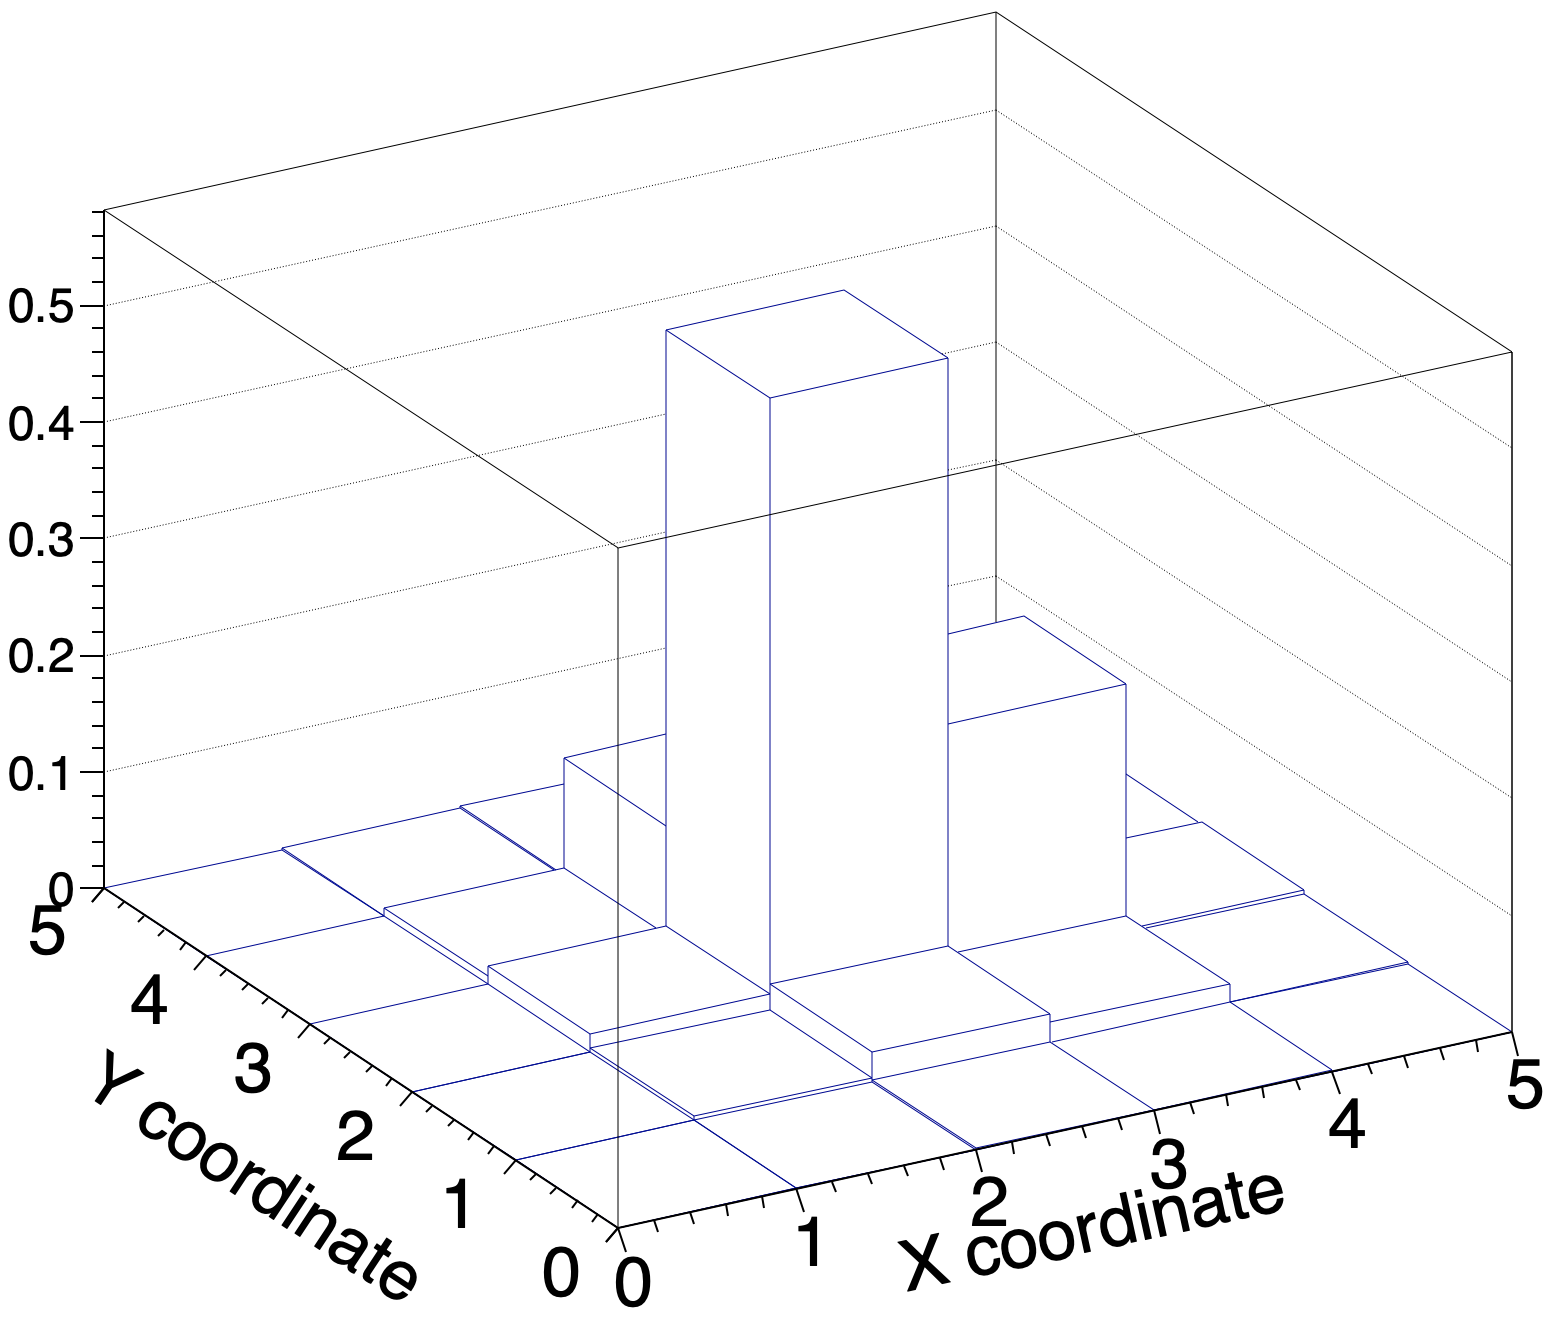
\includegraphics[width=1\linewidth]{images/z05.png}
  \caption{$z=0.5$}
  \label{fig:z05}
\end{subfigure}
\begin{subfigure}{.33\textwidth}
  \centering
  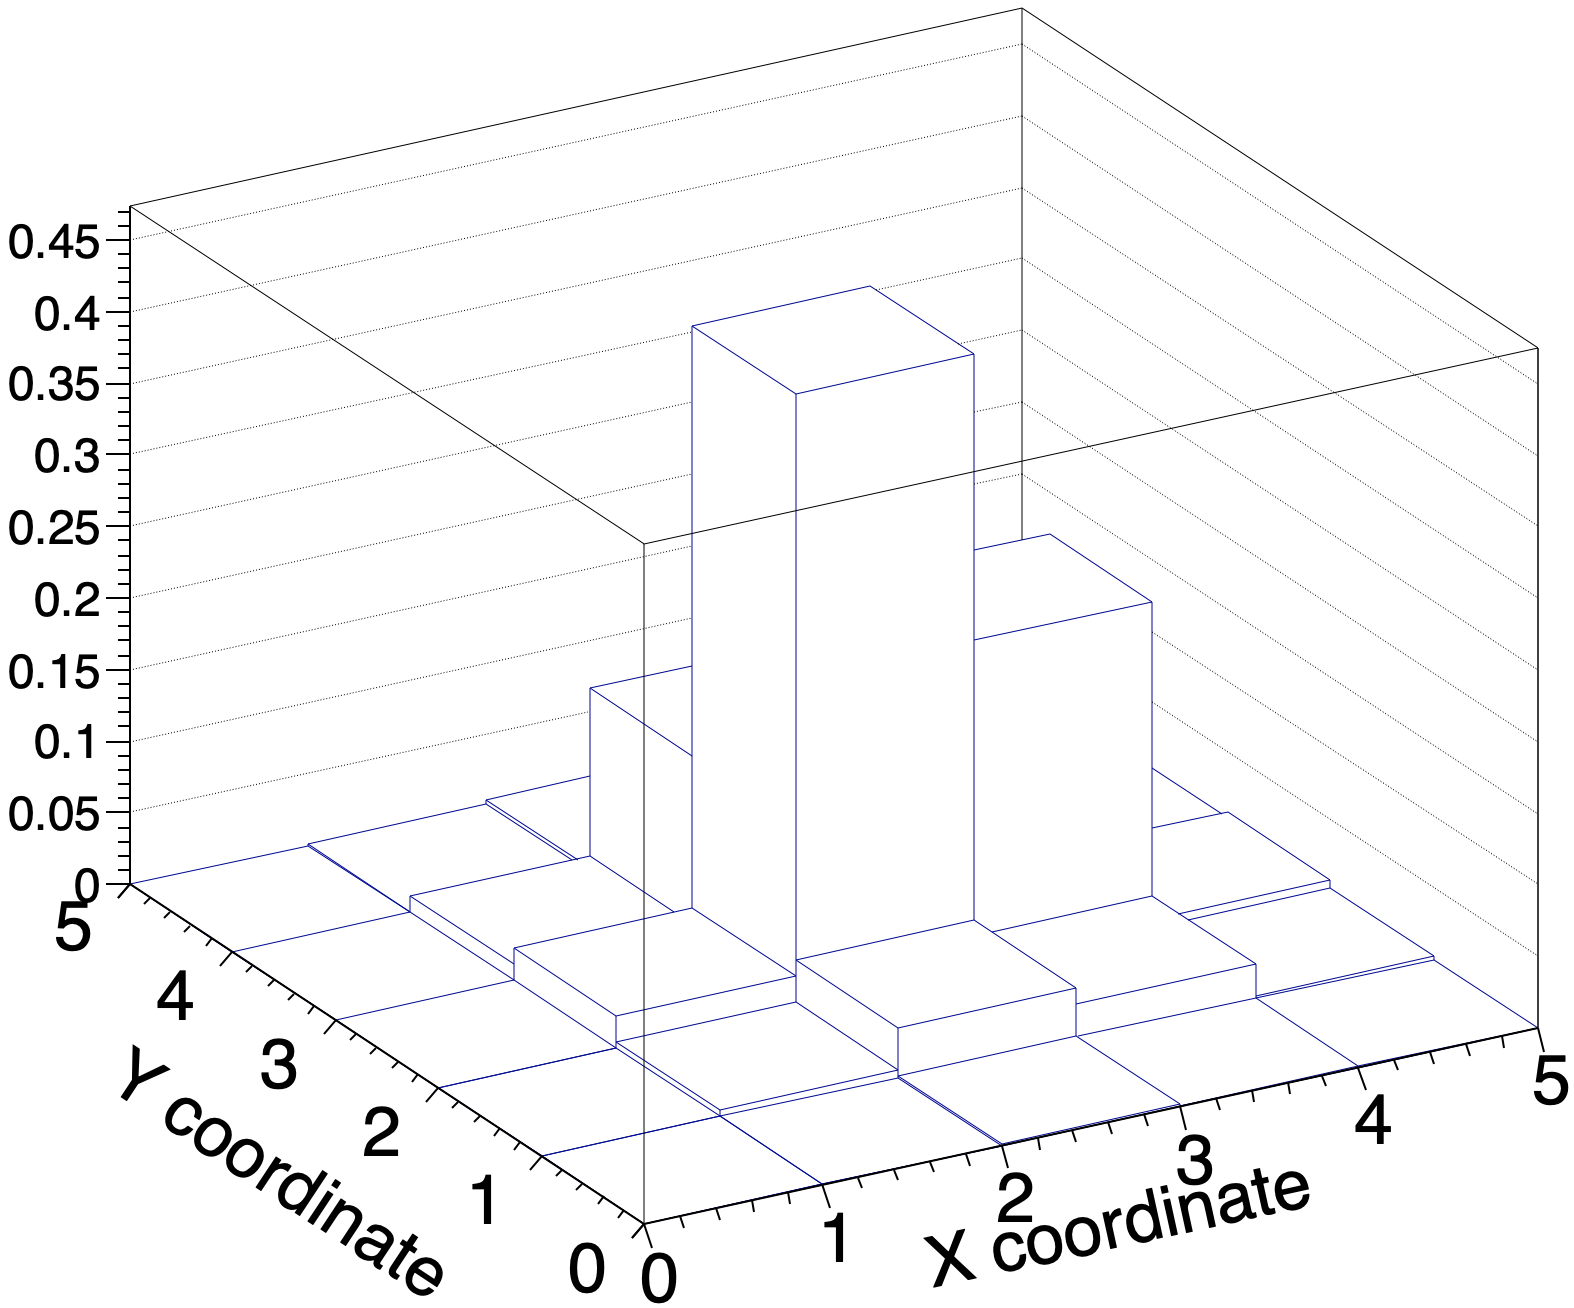
\includegraphics[width=1\linewidth]{images/z1.png}
  \caption{$z=1$}
  \label{fig:z1}
\end{subfigure}
\caption{Charge Distribution for $x=2.9$, $y=2.7$, and different $z$ coordinates}
\label{fig:z}
\end{figure}



%%%%%%%%%%%%%%%%%%%%%%%%%%%%%%%%%%%%%%%%%%%%%
%%%%%%%%%%%%%%%%%%%%%%%%%%%%%%%%%%%%%%%%%%%%%
\section{Conclusion}
We have written a C++ program that produces a theoretical charge distribution on $5\times 5$ grid for any original x-ray position according to a formula. Since this mathematical formula contains integrals and does not have an analytical solution, we have used various numerical methods to estimate the result.

We have also fitted two-dimensional Gaussian model to the charge distribution. The model is very accurate for our theoretical data because the distance between the predicted x-ray position and the original x-ray position is less that one tenth of a pixel in the vast majority of cases. In addition, we have found that the accuracy of the model strongly depends on the $z$ coordinate. This was expected because the amount of charge the neighboring pixels accumulate is dependant on the $z$ coordinate and the more charge the neighboring pixels accumulate, the more accurate our prediction is.

While our model estimates the original x-ray coordinate accurately, we have to keep in mind that the real data produced by an EMCCD camera are noisy and do not precisely reflect the theoretical distribution produced by the formula. Our EMCCD camera has 12\% signal amplitude fluctuations and cannot detect charge less than one electron. Therefore, when we apply our model to the real data, we are likely to get somewhat worse estimation accuracy.

In conclusion, our project will enable other scientist to study structure of various materials and see how the materials transform when you change its temperature or apply magnetic field. This is because if we can accurately measure the original x-ray coordinate, we can calculate the energy of the x-ray. The energy of the x-ray relates to the energy levels in the material which helps us see its structure.


\newpage
\bibliographystyle{alpha}
\bibliography{sample}
\sloppy

[1] Bisogni, V. National Synchrotron Light Source II. https://www.bnl.gov/nsls2/beamlines/beamline.php?r=2-ID

[2] Kotov, I. V., Li, J., Pelliciari, J., & Bisognia, V. (2022). Charge sharing in pixelated semiconductor sensors. Elsevier.



\end{document}